\chapter{Summary of  Developed Codes and Images}
\label{apendice2}

% In this appendix, the Section~\ref{appendice:technicalDrawings} illustrates the technical drawings regarding the development of the 3D device through the SolidWorks software.

% Already, for the Section~\ref{appendice:code}, it provides the link for the GitHub, where the user can find the documents developed. The files are divided as follows:
% % 
\begin{itemize}
    \item The project labeled WW4 incorporates a code base developed within the scope of this project. This serves as the crux of the program's interface, diligently overseeing the HTTP transactions essential to the project's operation. In addition, WW4 provides a range of complementary services, substantiating its comprehensive utility in the context of this project.
\end{itemize}

\clearpage
\section{Developed Codes }\label{appendice:code}

\begin{center}
    \href{https://github.com/iaggocapitanio1/woodWork4.0_API}{Github Repository for: WW4}
    \href{https://github.com/iaggocapitanio1/WoodWork40}{Github Repository for: System Architecture}
    \href{https://github.com/More-Collaborative-Laboratory/ww4zero}{Github Repository for: Data Model}
    \href{https://github.com/iaggocapitanio1/leftover-clientside}{Github Repository for: Jetson Client Side}
    \href{https://github.com/iaggocapitanio1/WW4FileFinder}{Github Repository for: FileSystem Media Superviser}
    \href{https://github.com/iaggocapitanio1/WWWatcher}{Github Repository for: FileSystem CutLists Superviser}
\end{center}


\section{Images}
The following images, included in this appendix, were used as the primary source for the data set upon which our statistical analysis was conducted. These images were captured under controlled conditions to ensure accuracy and consistency across all measurements. Each image illustrates a specific dimension - width and height, which were measured using state-of-the-art measurement tools. These measurements were then collated to form the data set, which was subsequently used to calculate the standard deviation and systematic error. 


\subsection{Systematic Error Images}
\begin{figure}[H]
    \centering
    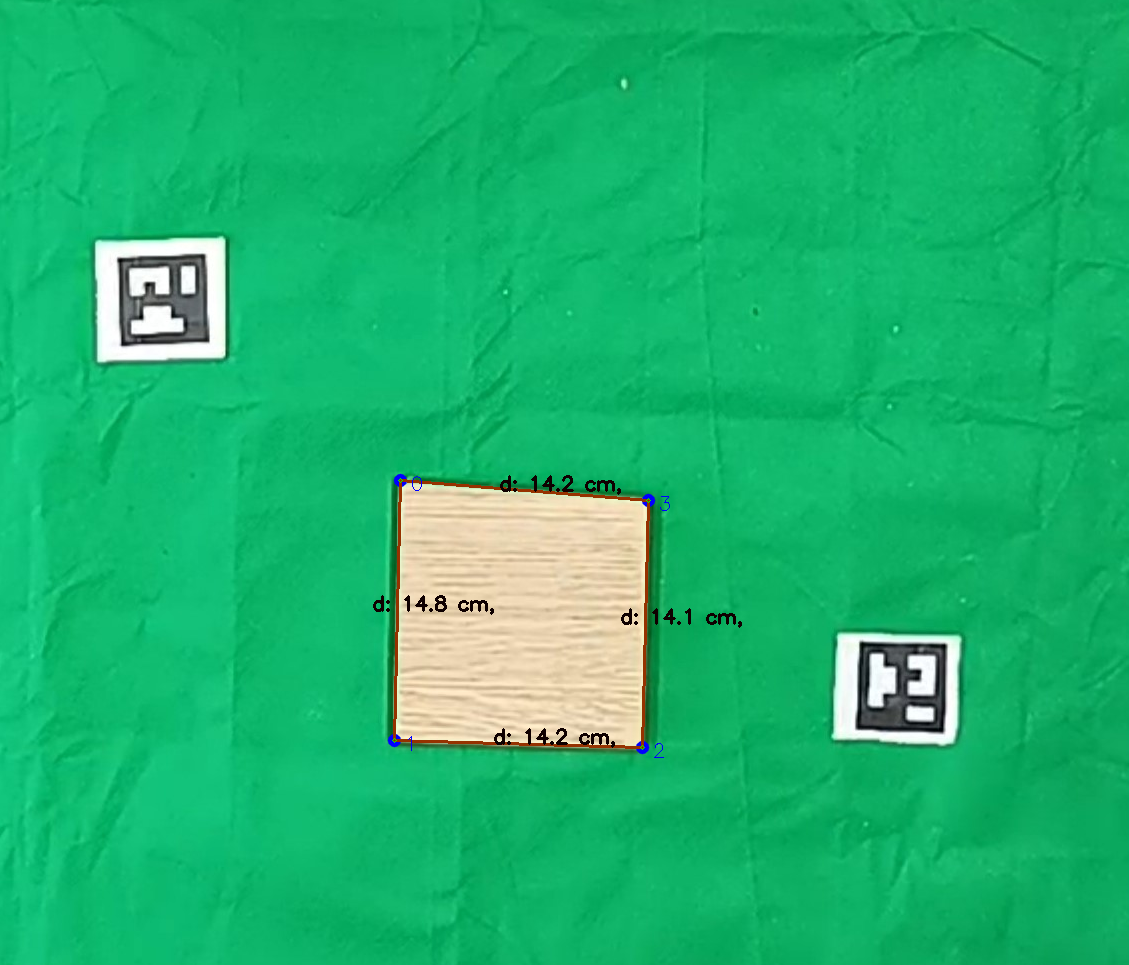
\includegraphics[width=0.35\linewidth]{images/Systematic/14.5x14.3.png}
    \caption{Wood Piece with 14.5 x 14.2}
    \label{fig:enter-label}
\end{figure}

\begin{figure}[H]
    \centering
    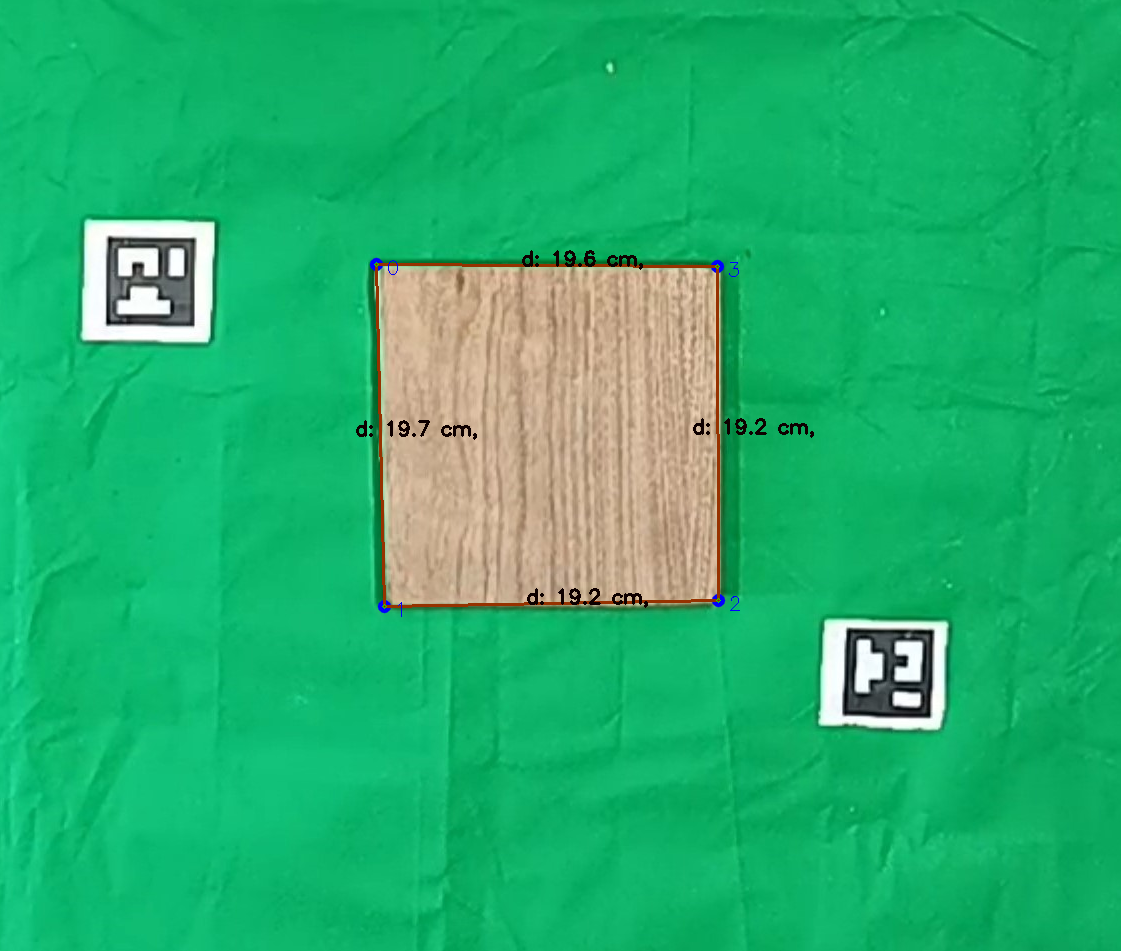
\includegraphics[width=0.35\linewidth]{images/Systematic/19.5x19.4.png}
    \caption{Wood Piece with 19.5 x 19.4}
    \label{fig:enter-label}
\end{figure}



\begin{figure}[H]
    \centering
    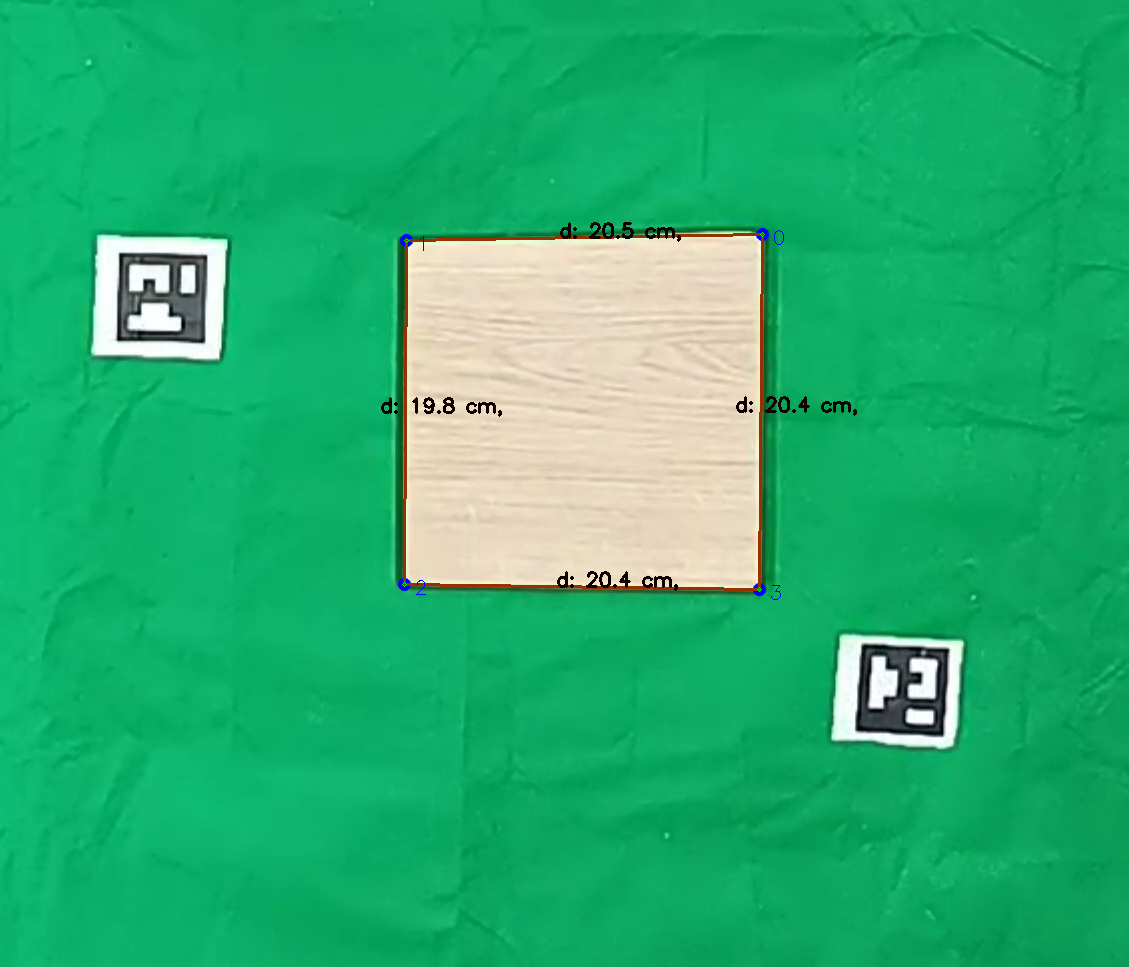
\includegraphics[width=0.35\linewidth]{images/Systematic/20.5x20.3.png}
    \caption{Wood Piece with 20.5 x 20.3}
    \label{fig:enter-label}
\end{figure}



\begin{figure}[H]
    \centering
    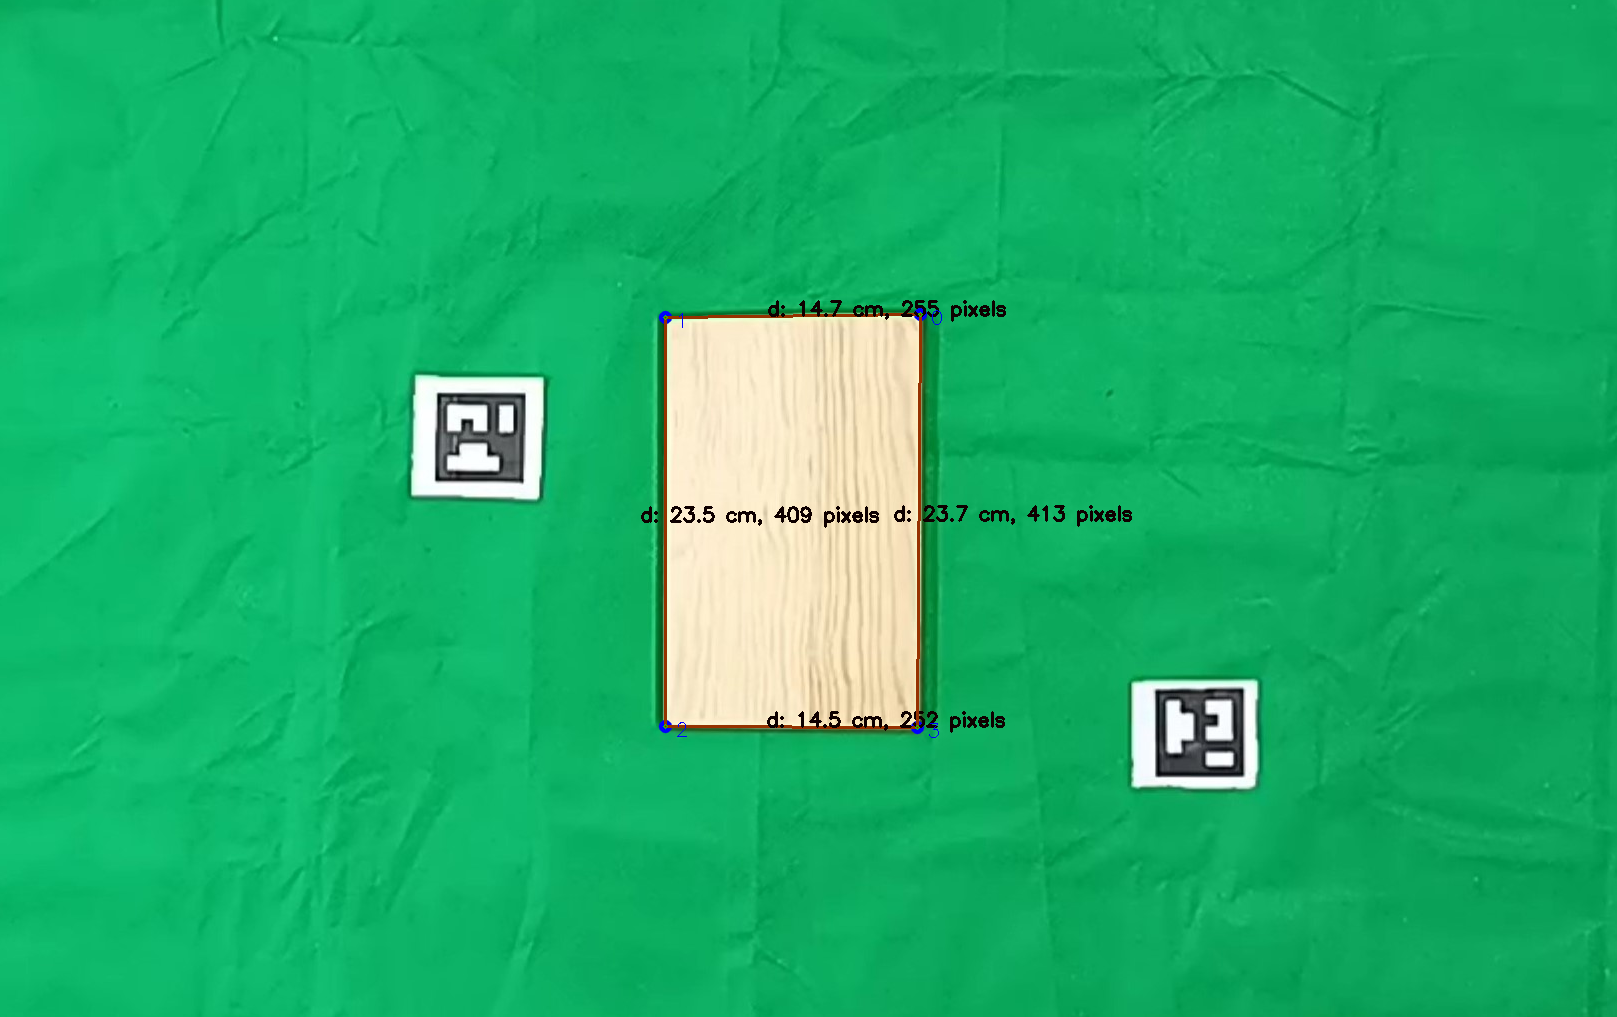
\includegraphics[width=0.35\linewidth]{images/Systematic/23.6x14.6.png}
    \caption{Wood Piece with 23.6 x 14.6}
    \label{fig:enter-label}
\end{figure}



\begin{figure}[H]
    \centering
    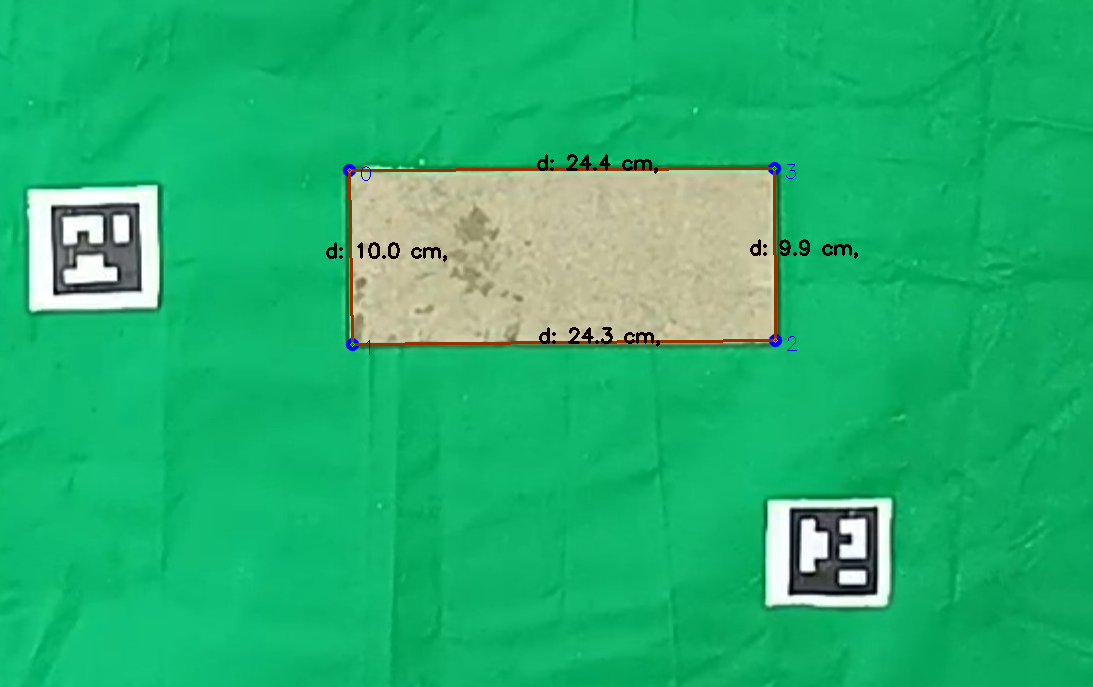
\includegraphics[width=0.35\linewidth]{images/Systematic/24.5x10.png}
    \caption{Wood Piece with 24.5 x 10}
    \label{fig:enter-label}
\end{figure}


\begin{figure}[H]
    \centering
    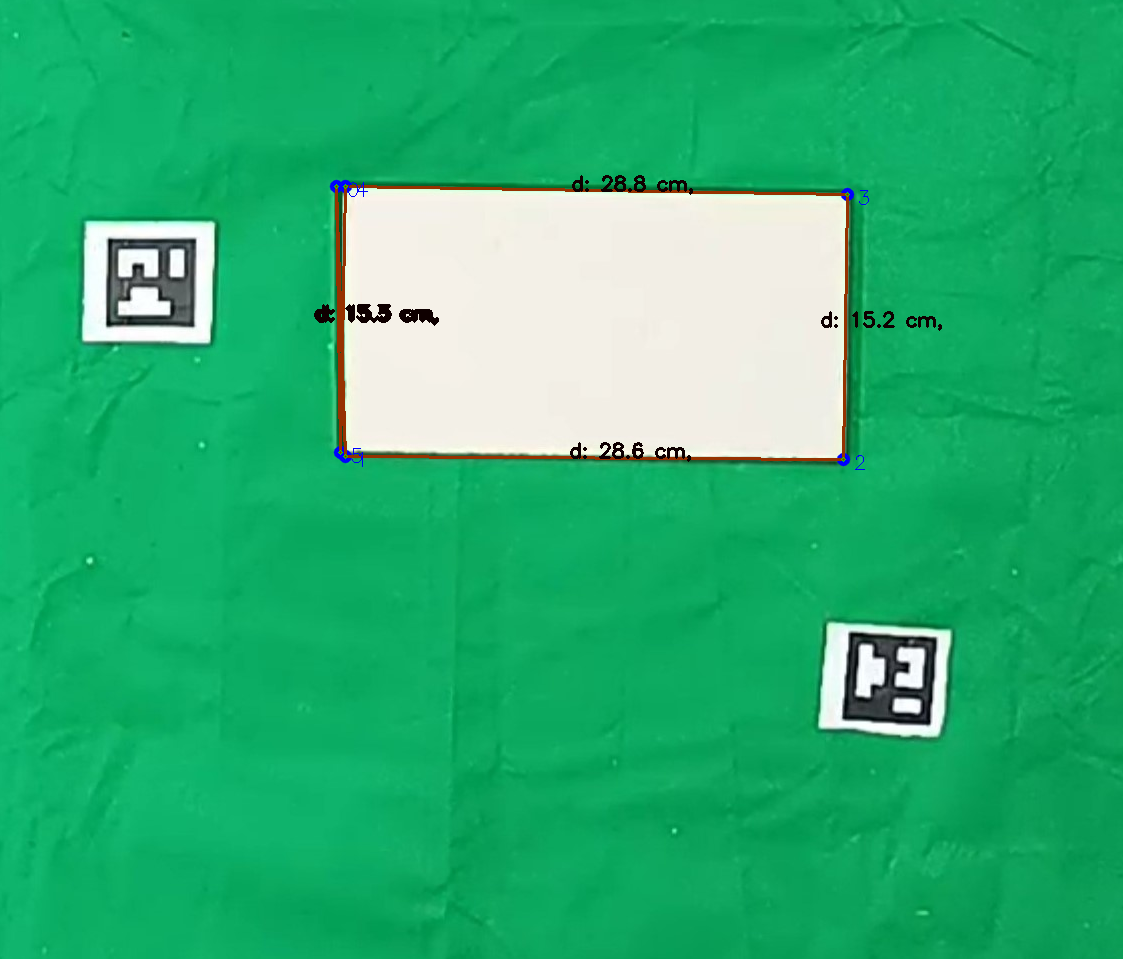
\includegraphics[width=0.35\linewidth]{images/Systematic/28.9x15.2.png}
    \caption{Wood Piece with 28.9 x 15.2}
    \label{fig:enter-label}
\end{figure}


\begin{figure}[H]
    \centering
    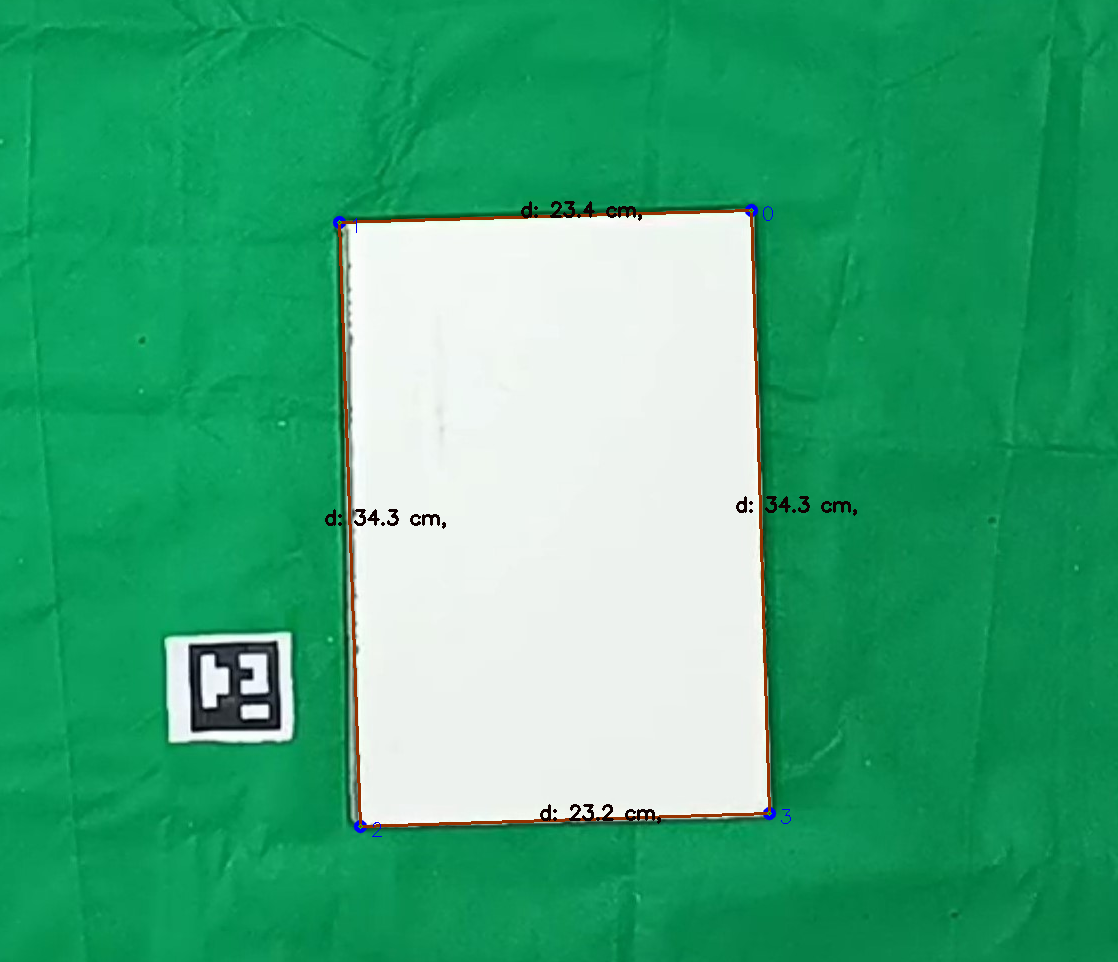
\includegraphics[width=0.35\linewidth]{images/Systematic/34.3x23.3.png}
    \caption{Wood Piece with 34.3 x 23.3}
    \label{fig:enter-label}
\end{figure}


\begin{figure}[H]
    \centering
    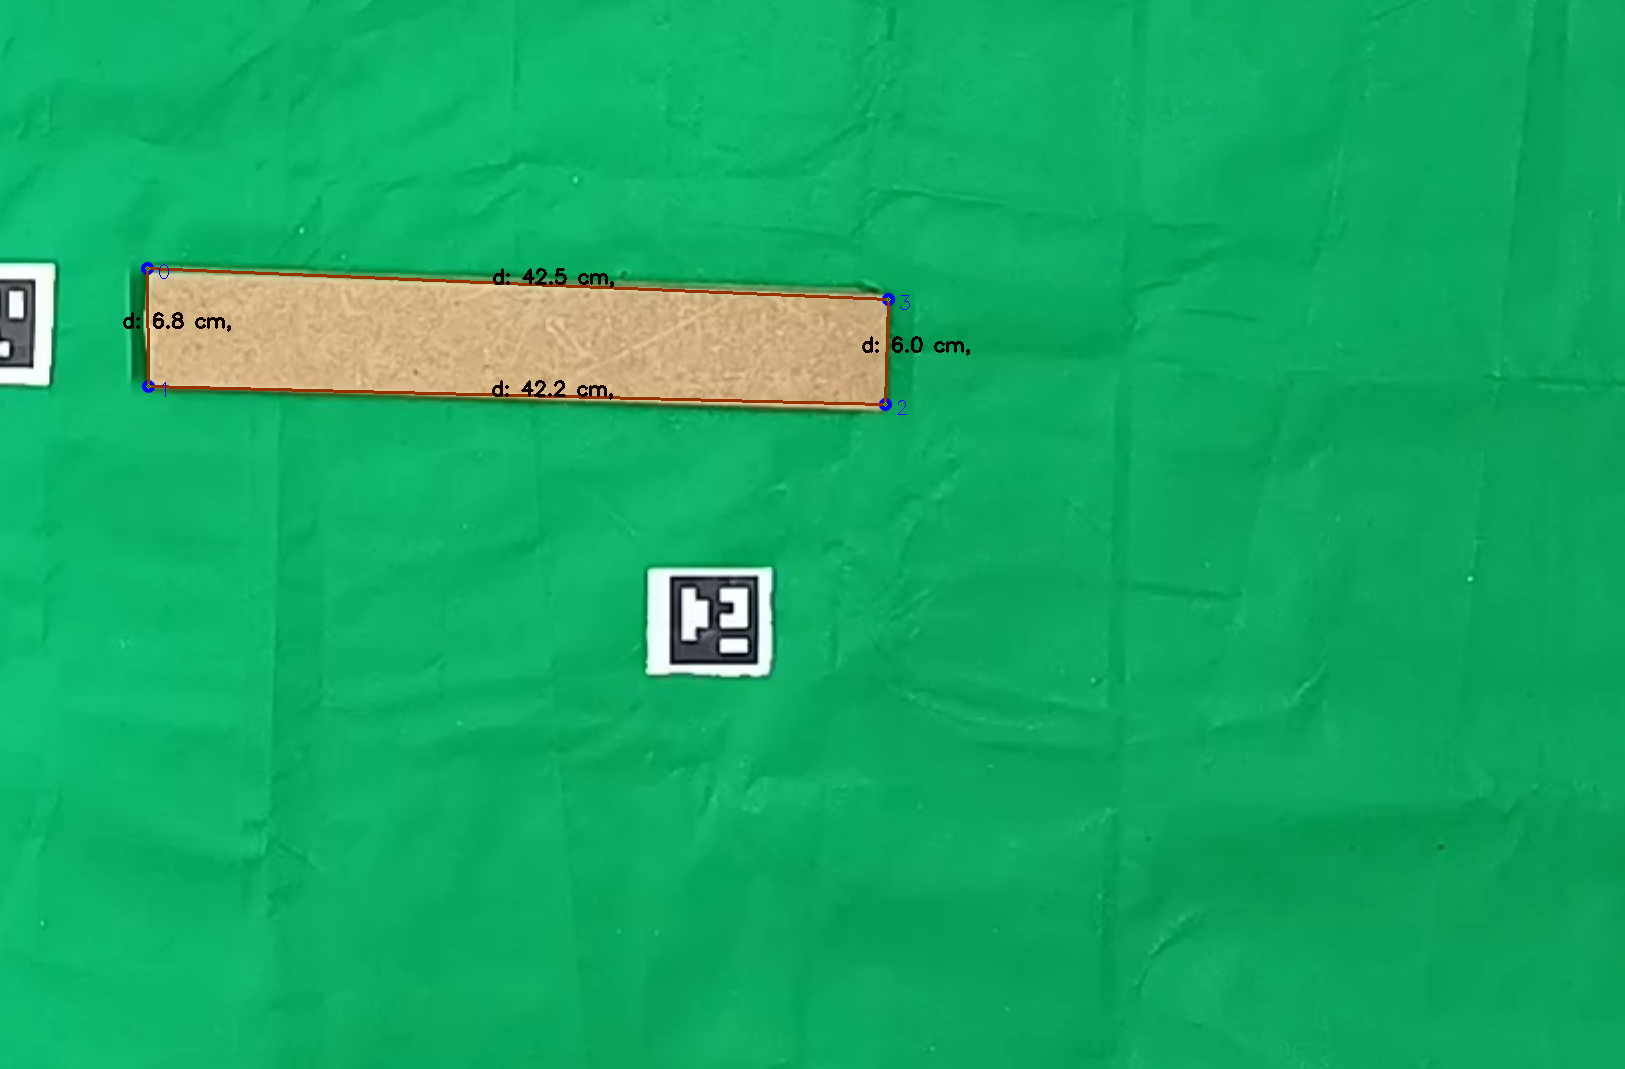
\includegraphics[width=0.35\linewidth]{images/Systematic/42.5x6.2.png}
    \caption{Wood Piece with 42.5 x 6.2}
    \label{fig:enter-label}
\end{figure}


\begin{figure}[H]
    \centering
    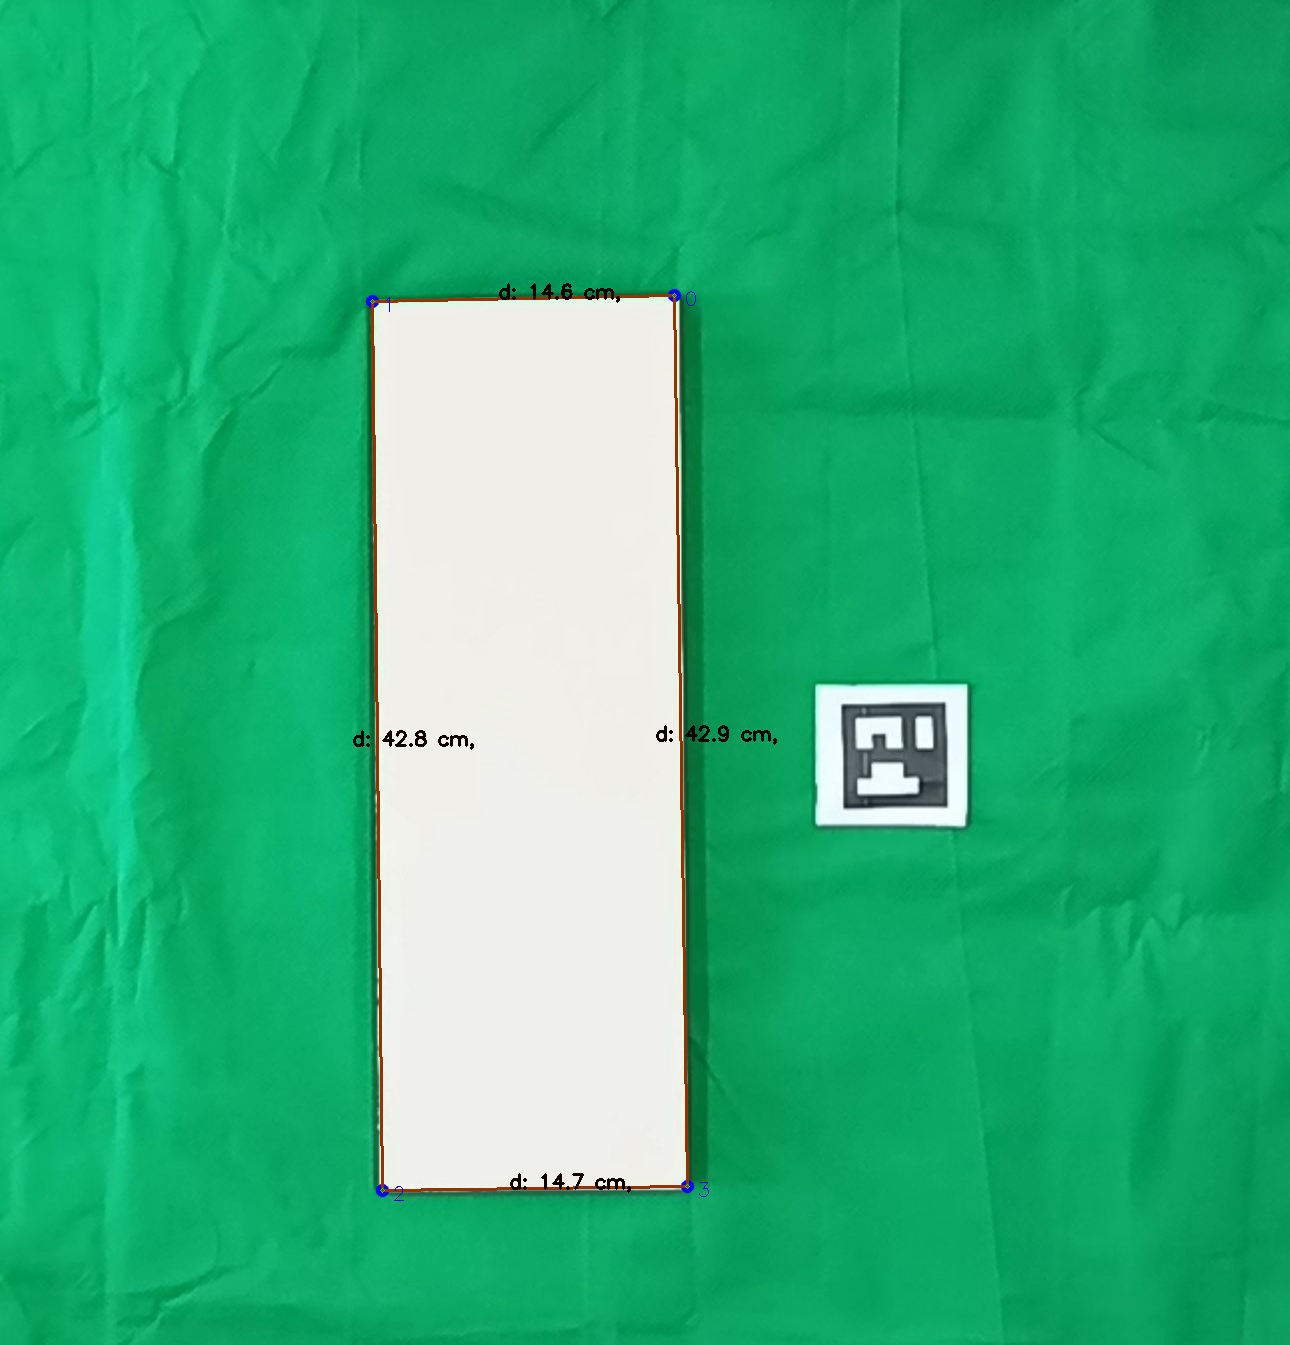
\includegraphics[width=0.35\linewidth]{images/Systematic/43x14.9.png}
    \caption{Wood Piece with 43 x 14.9}
    \label{fig:enter-label}
\end{figure}


\begin{figure}[H]
    \centering
    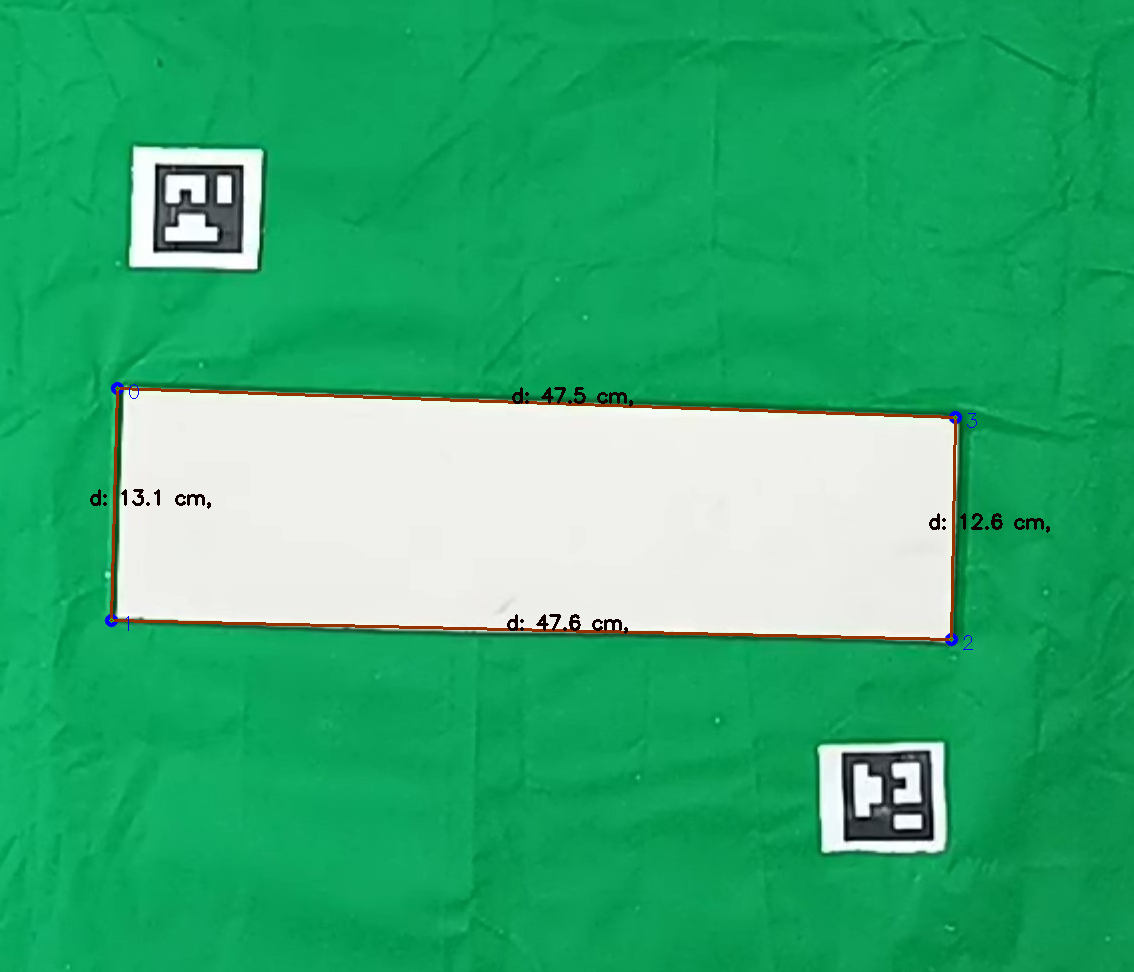
\includegraphics[width=0.35\linewidth]{images/Systematic/47.5x13.png}
    \caption{Wood Piece with 47.5 x 13}
    \label{fig:enter-label}
\end{figure}



\subsection{Standard Deviation Images}

\begin{figure}[!h]
    \centering
    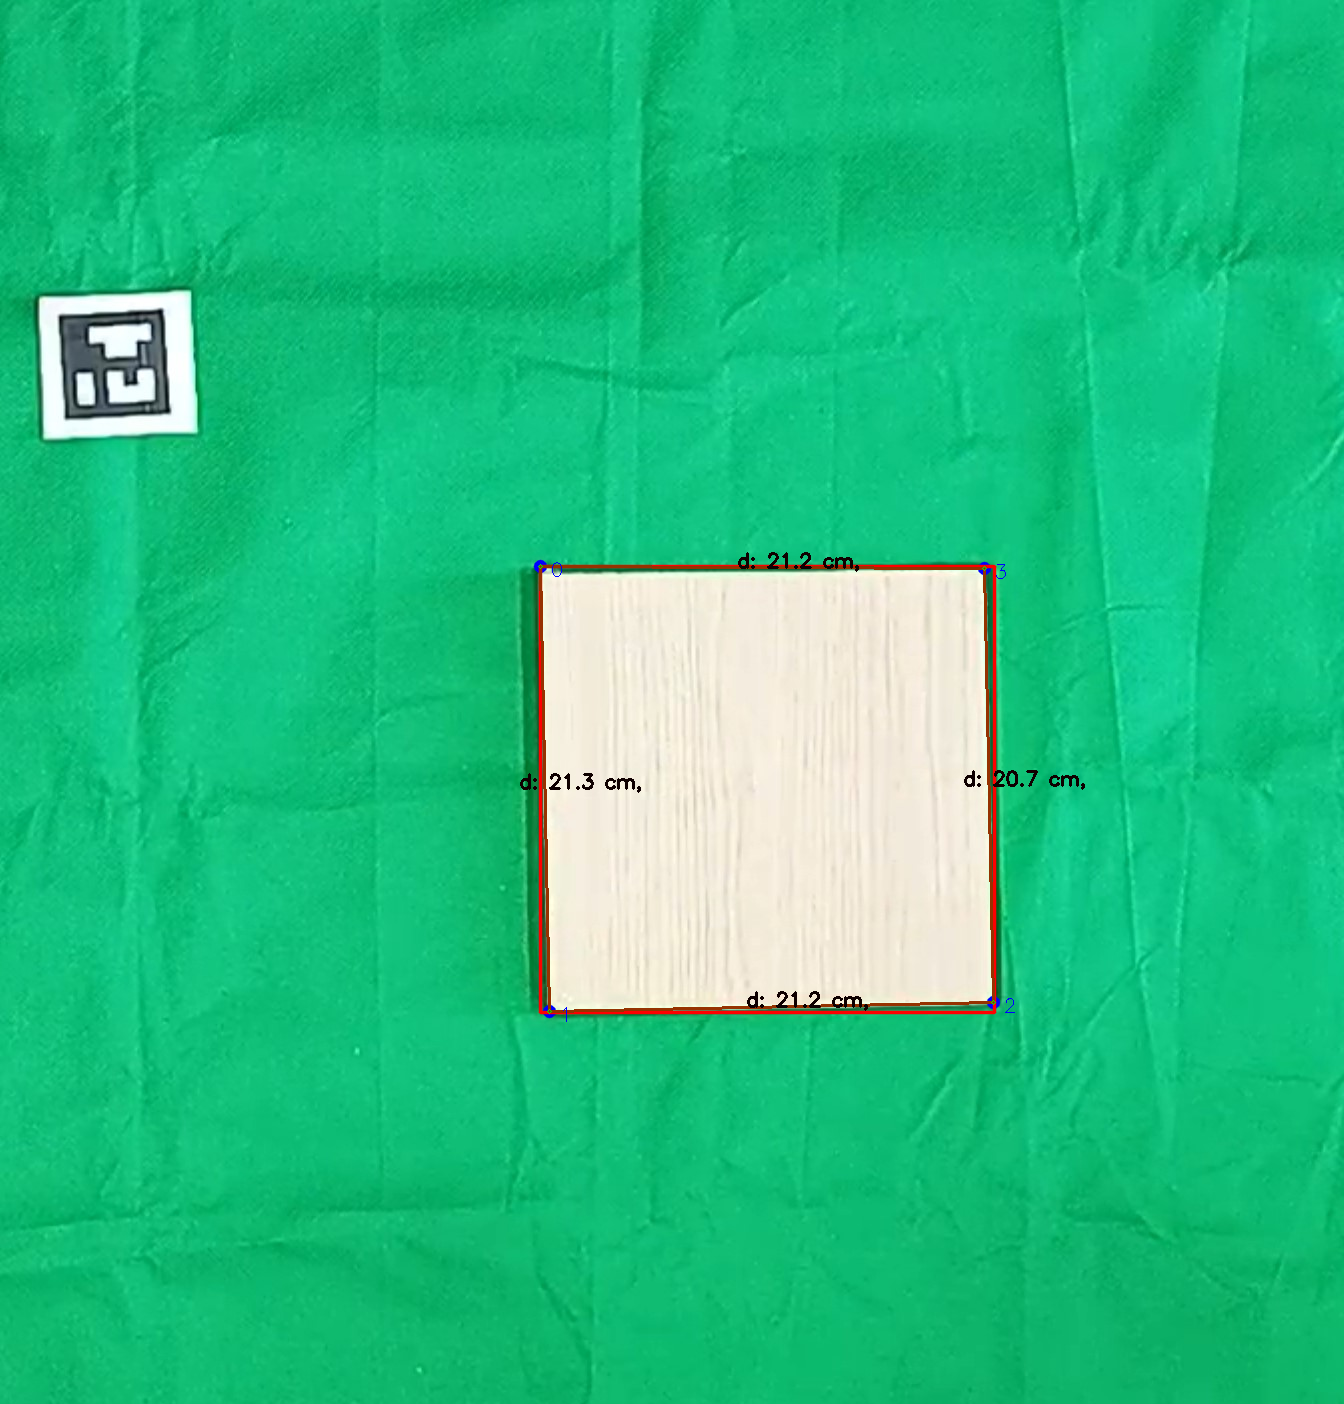
\includegraphics[width=0.35\linewidth]{images/Normal Dist/21.2x21_1.png}
    \caption{Wood Piece with 21.2 x 21}
    \label{fig:enter-label}
\end{figure}

\begin{figure}[!h]
    \centering
    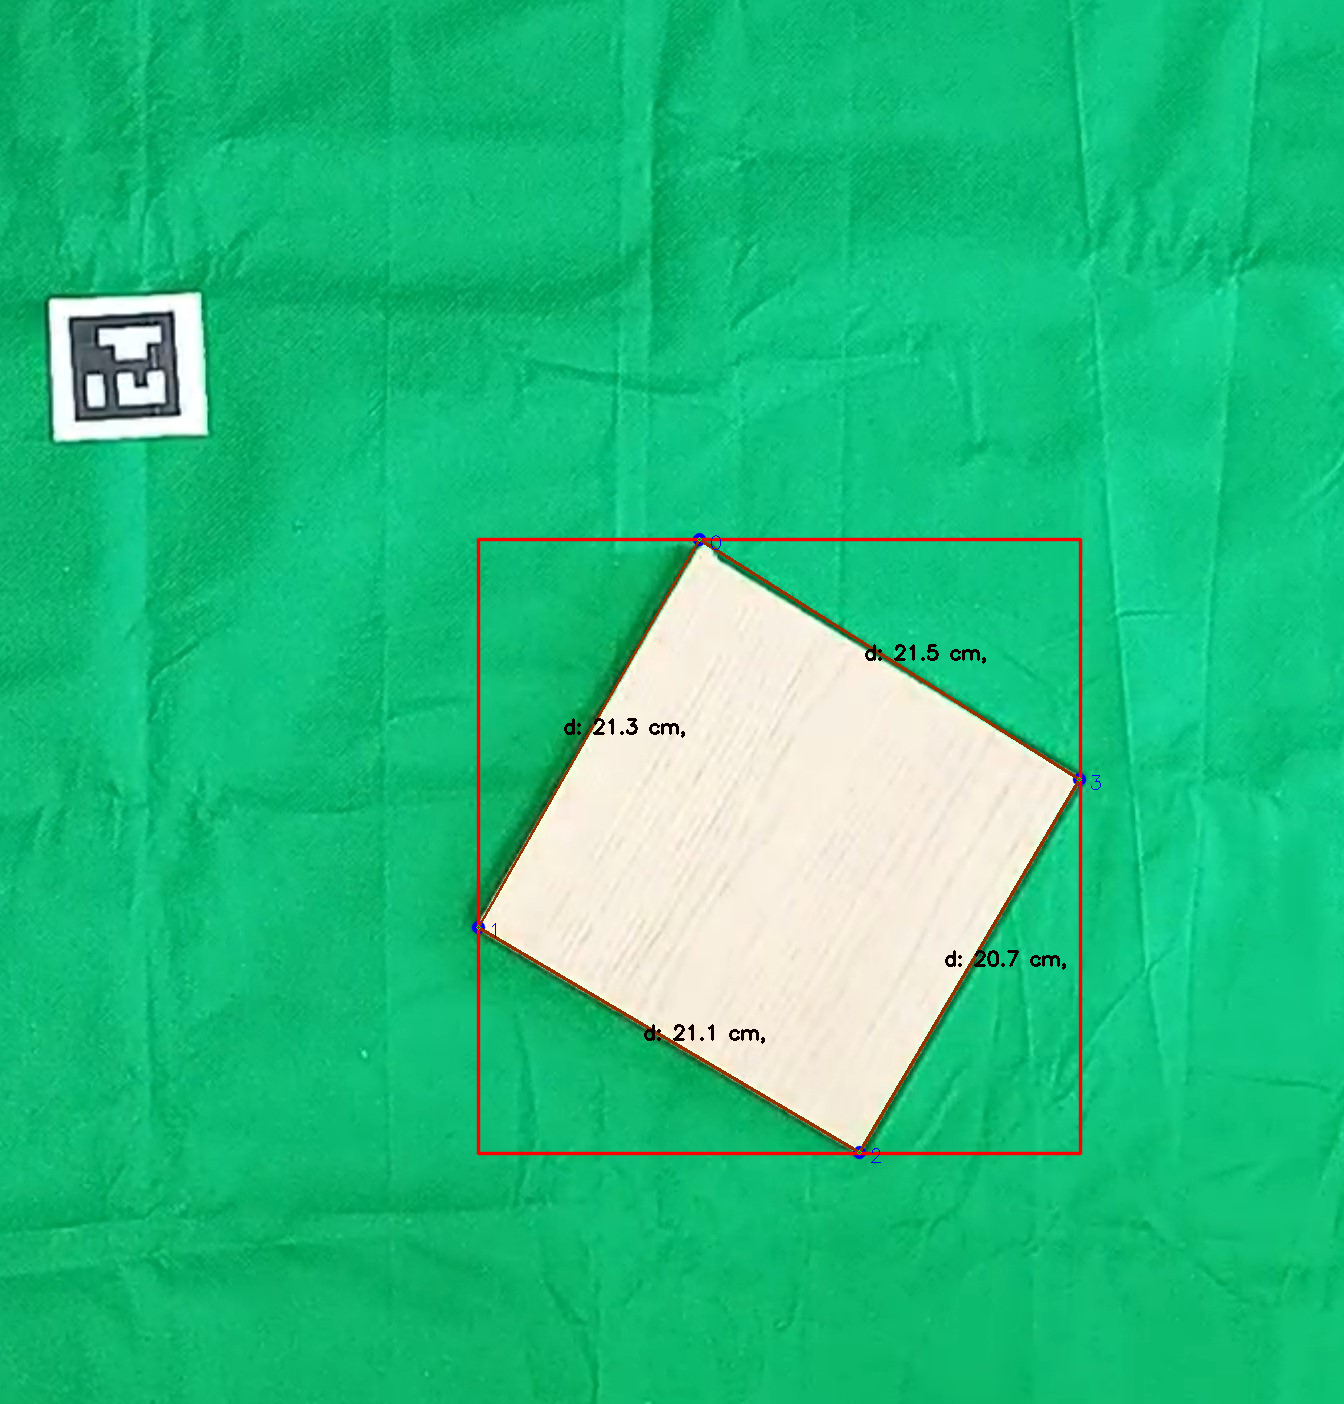
\includegraphics[width=0.35\linewidth]{images/Normal Dist/21.2x21_2.png}
    \caption{Wood Piece with 21.3 x 21}
    \label{fig:enter-label}
\end{figure}


\begin{figure}[!h]
    \centering
    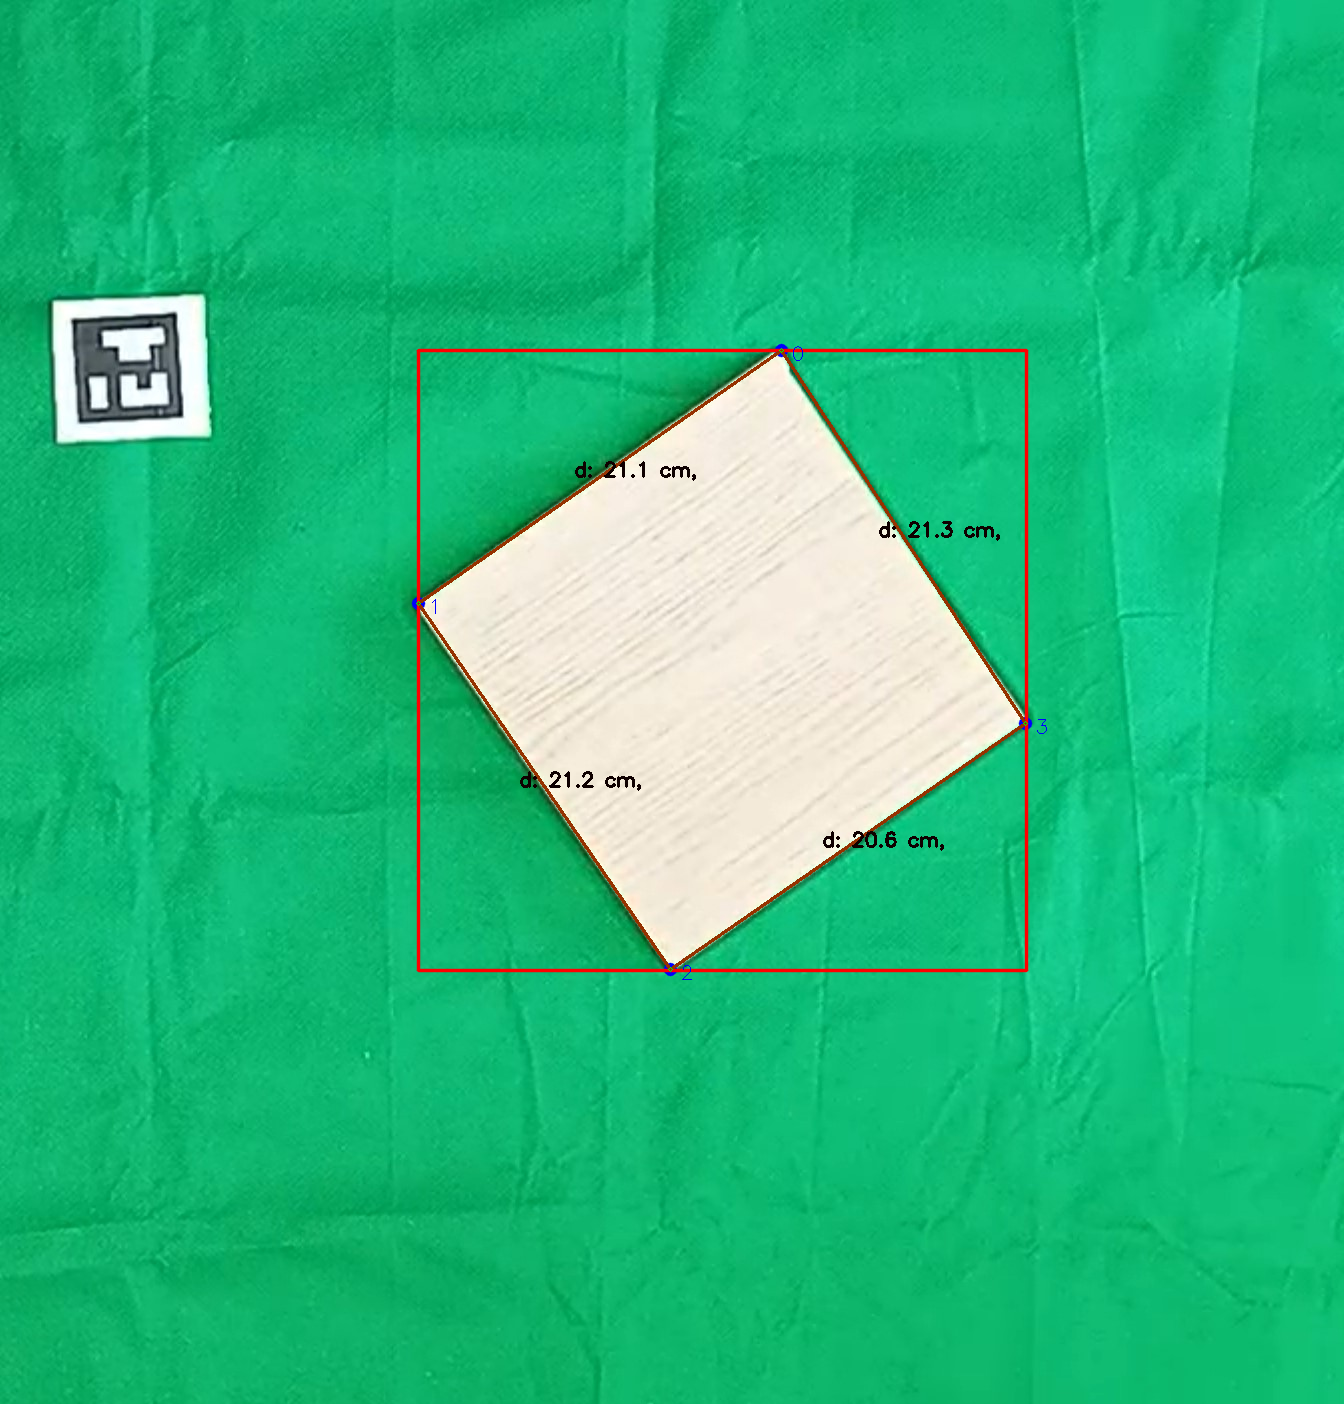
\includegraphics[width=0.35\linewidth]{images/Normal Dist/21.2x21_3.png}
    \caption{Wood Piece with 21.25 x 20.85}
    \label{fig:enter-label}
\end{figure}


\begin{figure}[!h]
    \centering
    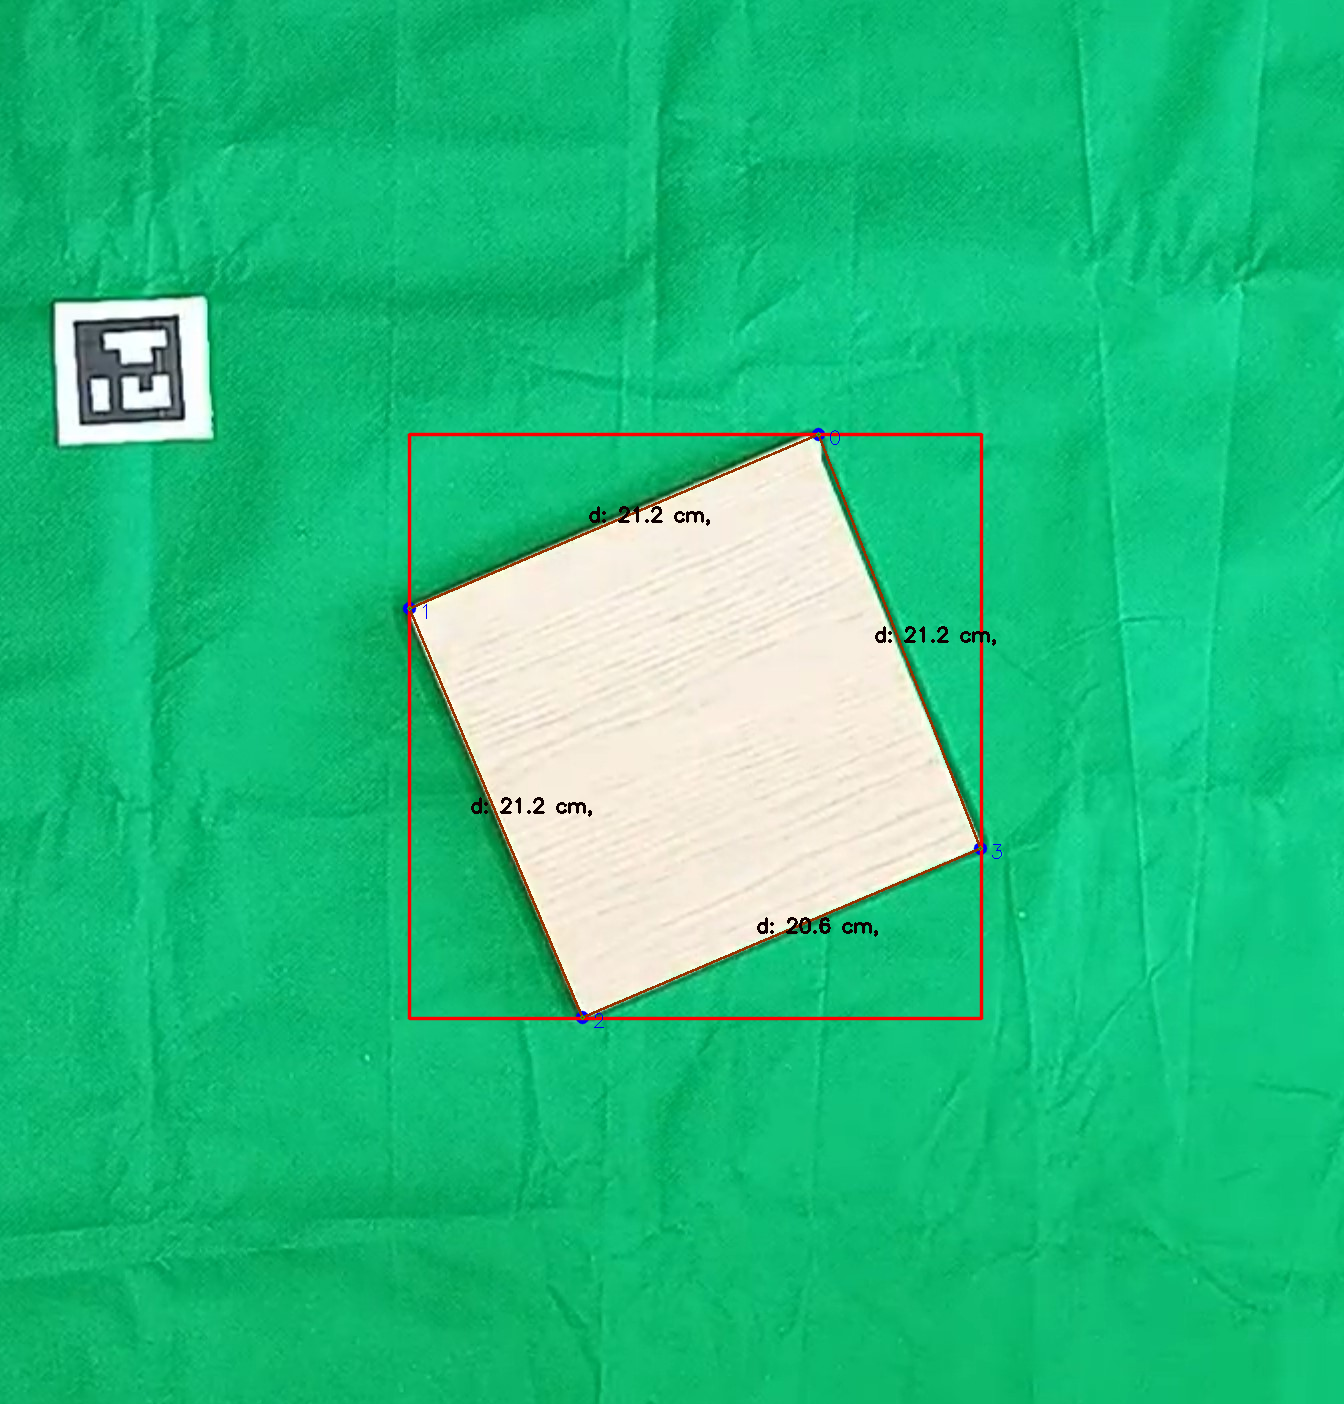
\includegraphics[width=0.35\linewidth]{images/Normal Dist/21.2x21_4.png}
    \caption{Wood Piece with 21.2 x 20.85}
    \label{fig:enter-label}
\end{figure}


\begin{figure}[!h]
    \centering
    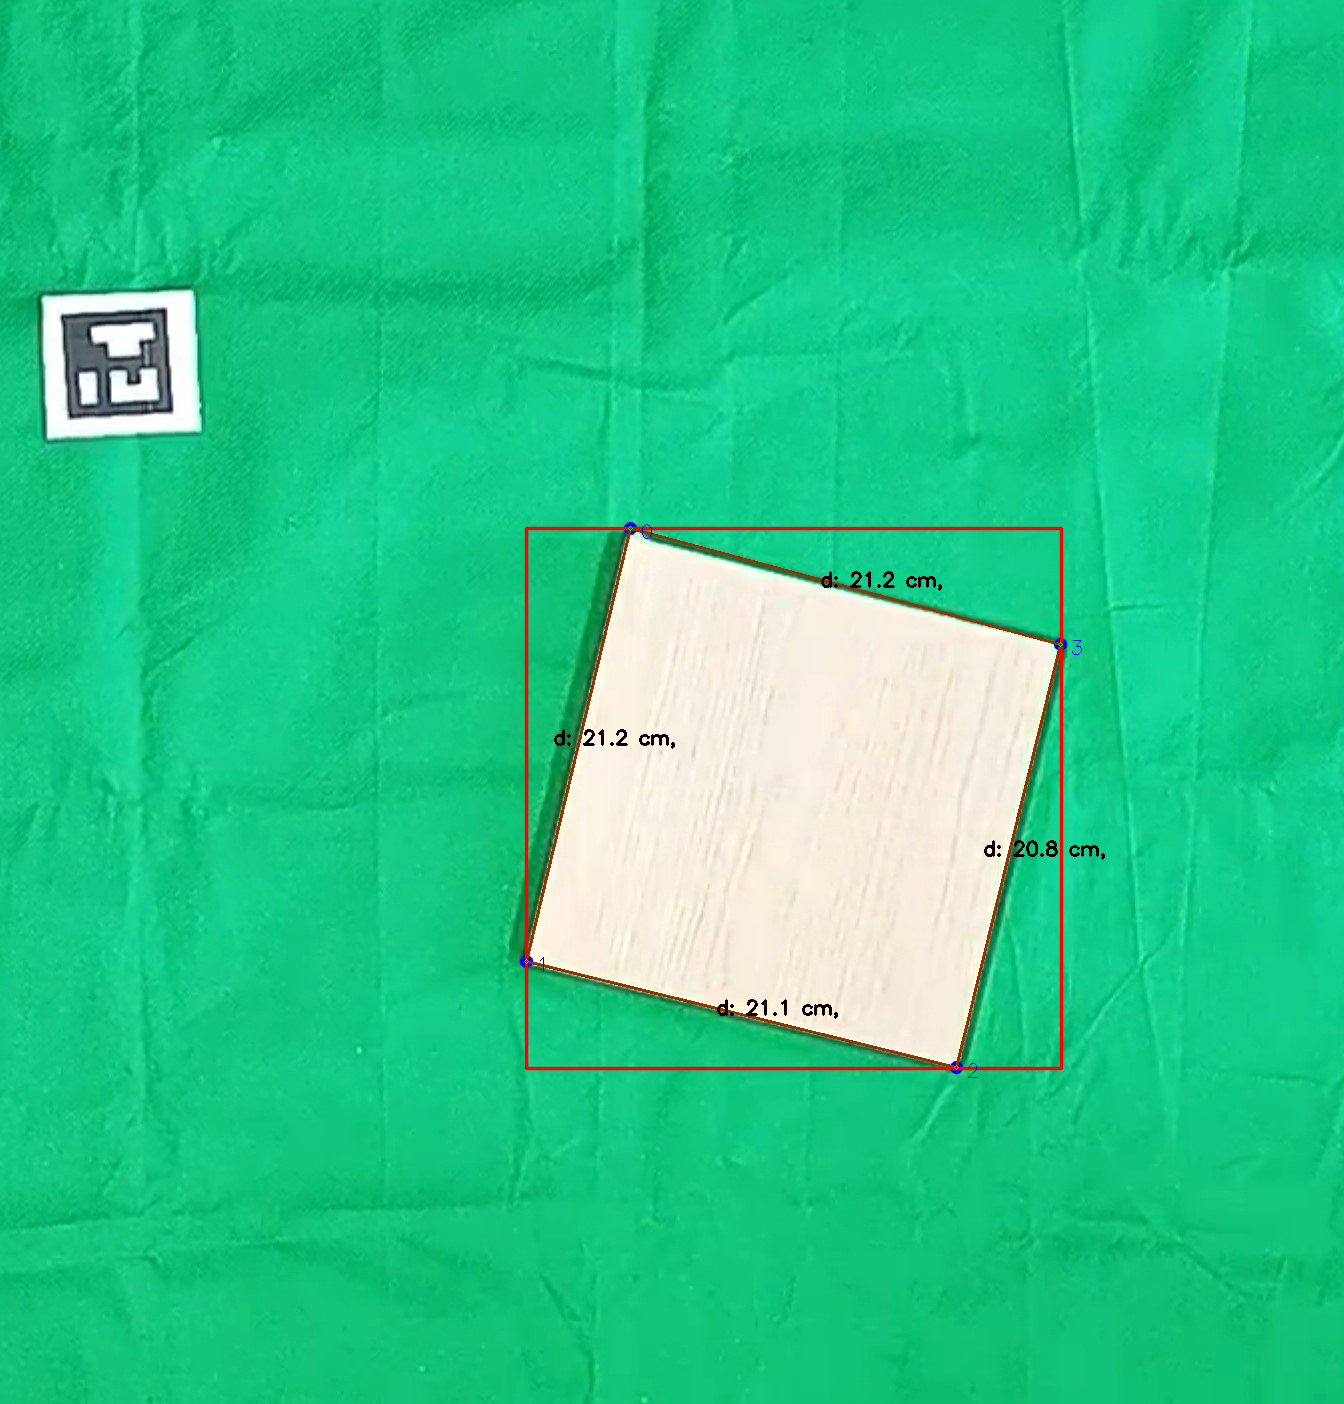
\includegraphics[width=0.35\linewidth]{images/Normal Dist/21.2x21_5.png}
    \caption{Wood Piece with 21.25 x 21}
    \label{fig:enter-label}
\end{figure}


\begin{figure}[!h]
    \centering
    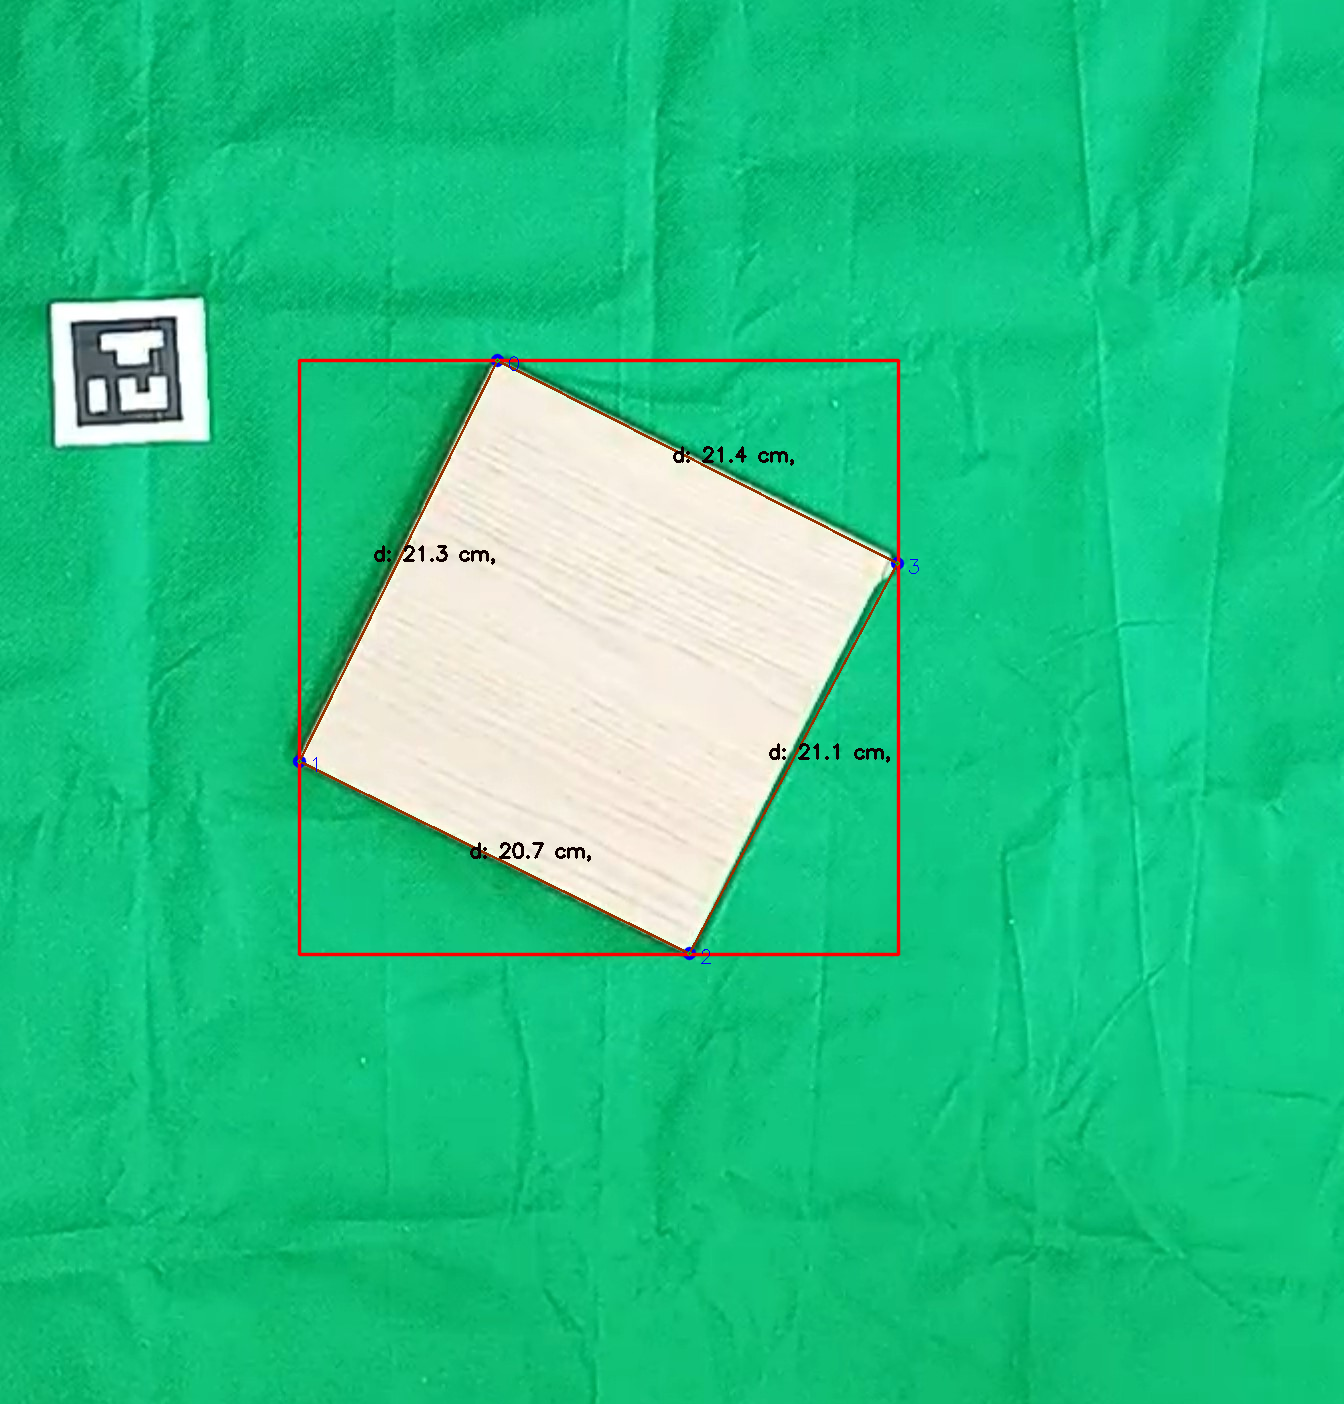
\includegraphics[width=0.35\linewidth]{images/Normal Dist/21.2x21_6.png}
    \caption{Wood Piece with 21.2 x 21.05}
    \label{fig:enter-label}
\end{figure}




\begin{figure}[!h]
    \centering
    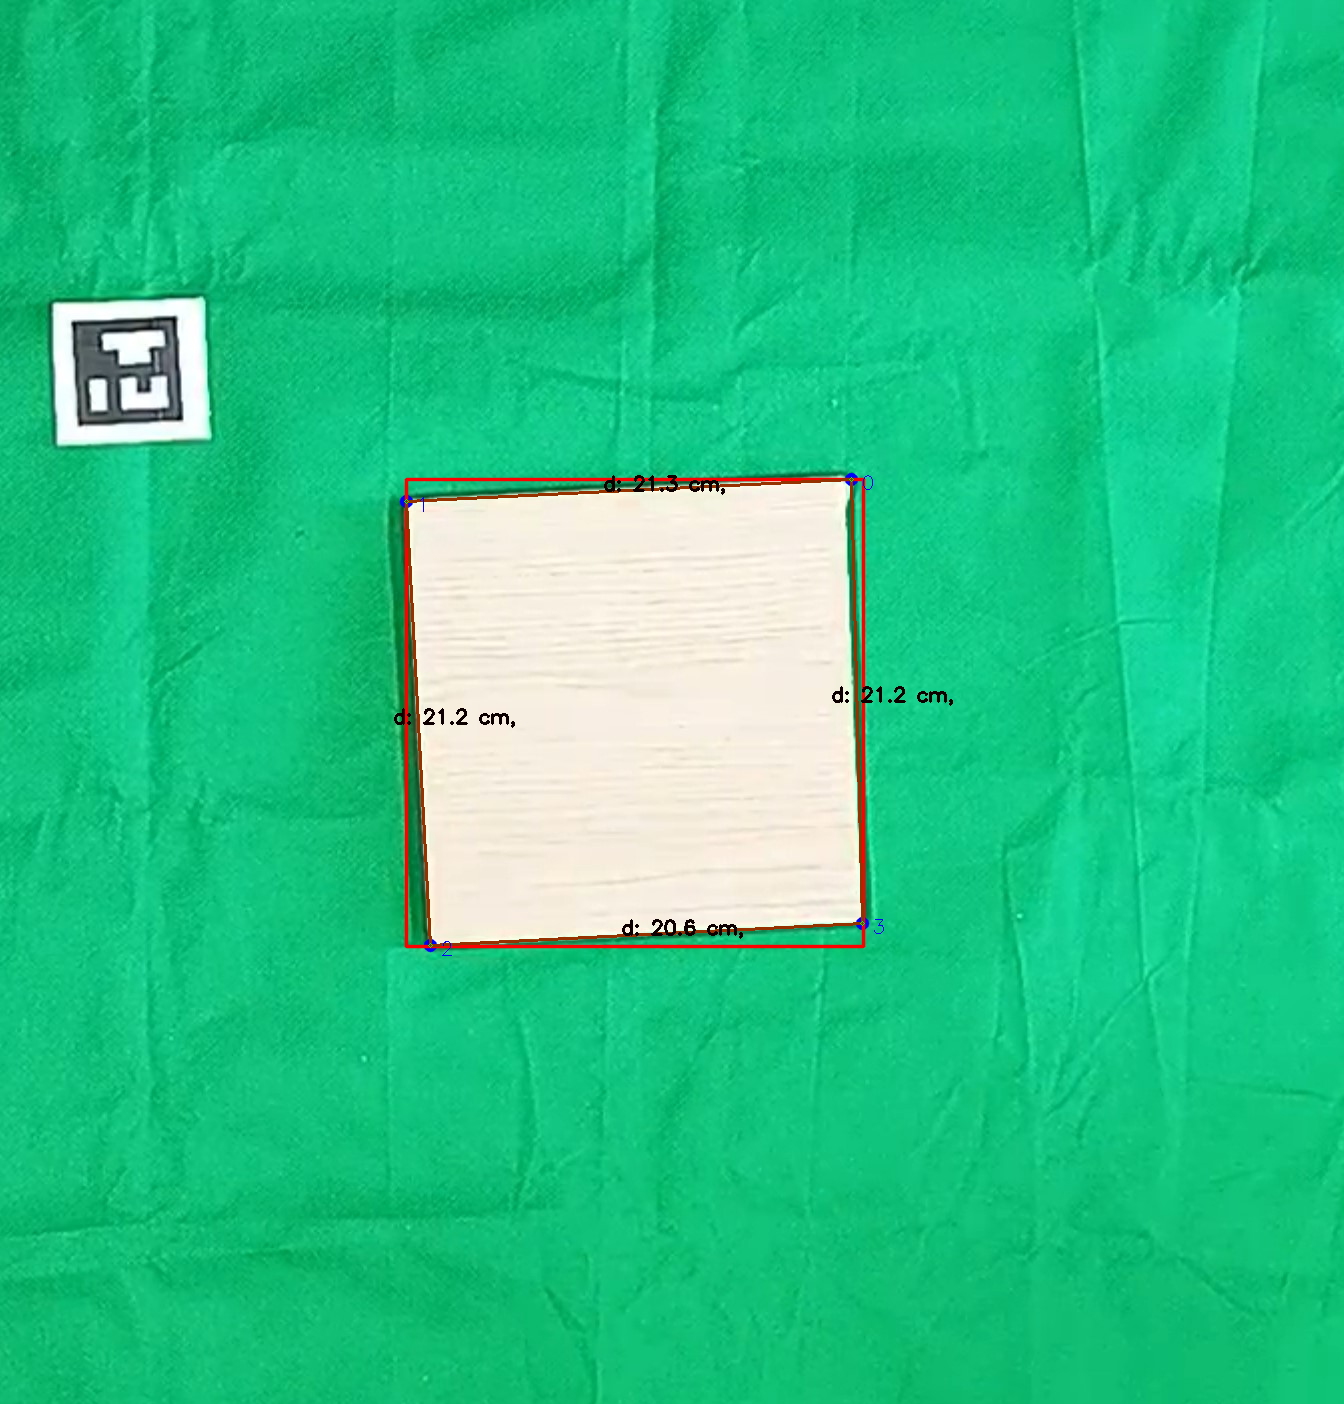
\includegraphics[width=0.35\linewidth]{images/Normal Dist/21.2x21_7.png}
    \caption{Wood Piece with 21.2 x 20.95}
    \label{fig:enter-label}
\end{figure}


\begin{figure}[!h]
    \centering
    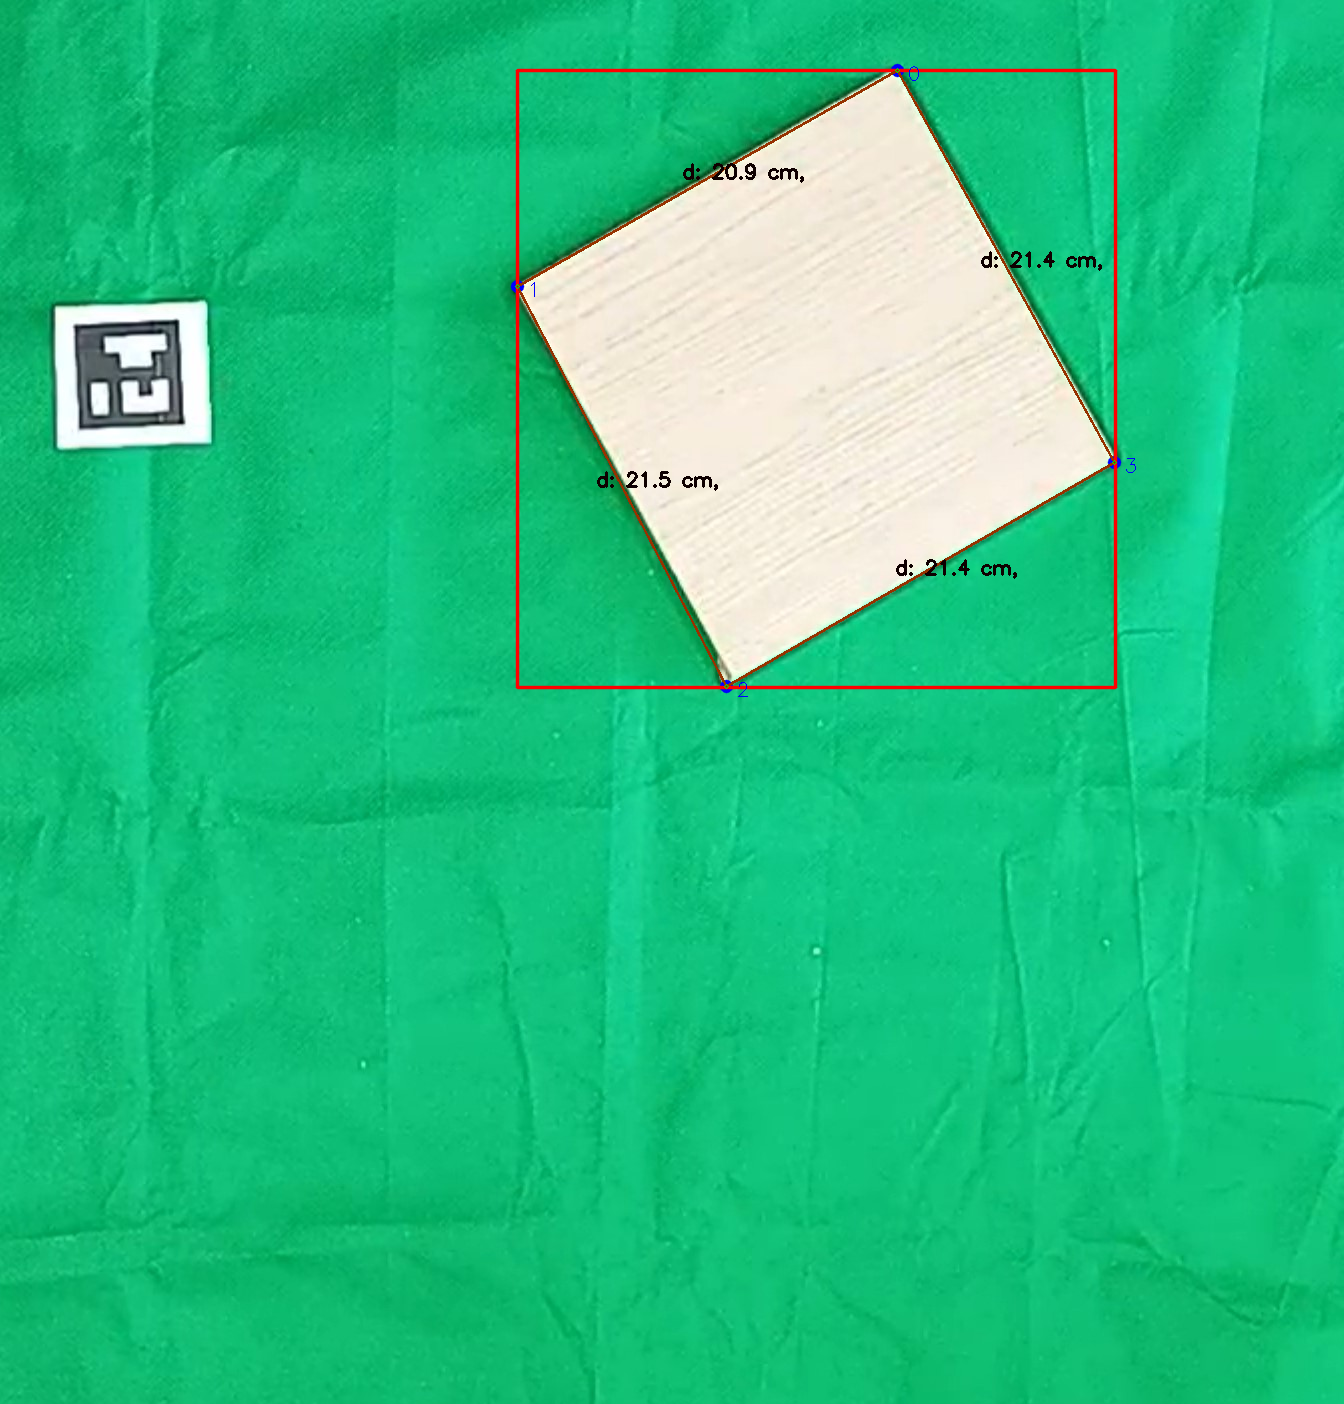
\includegraphics[width=0.35\linewidth]{images/Normal Dist/21.2x21_8.png}
    \caption{Wood Piece with 21.45 x 21.15}
    \label{fig:enter-label}
\end{figure}



\begin{figure}[!h]
    \centering
    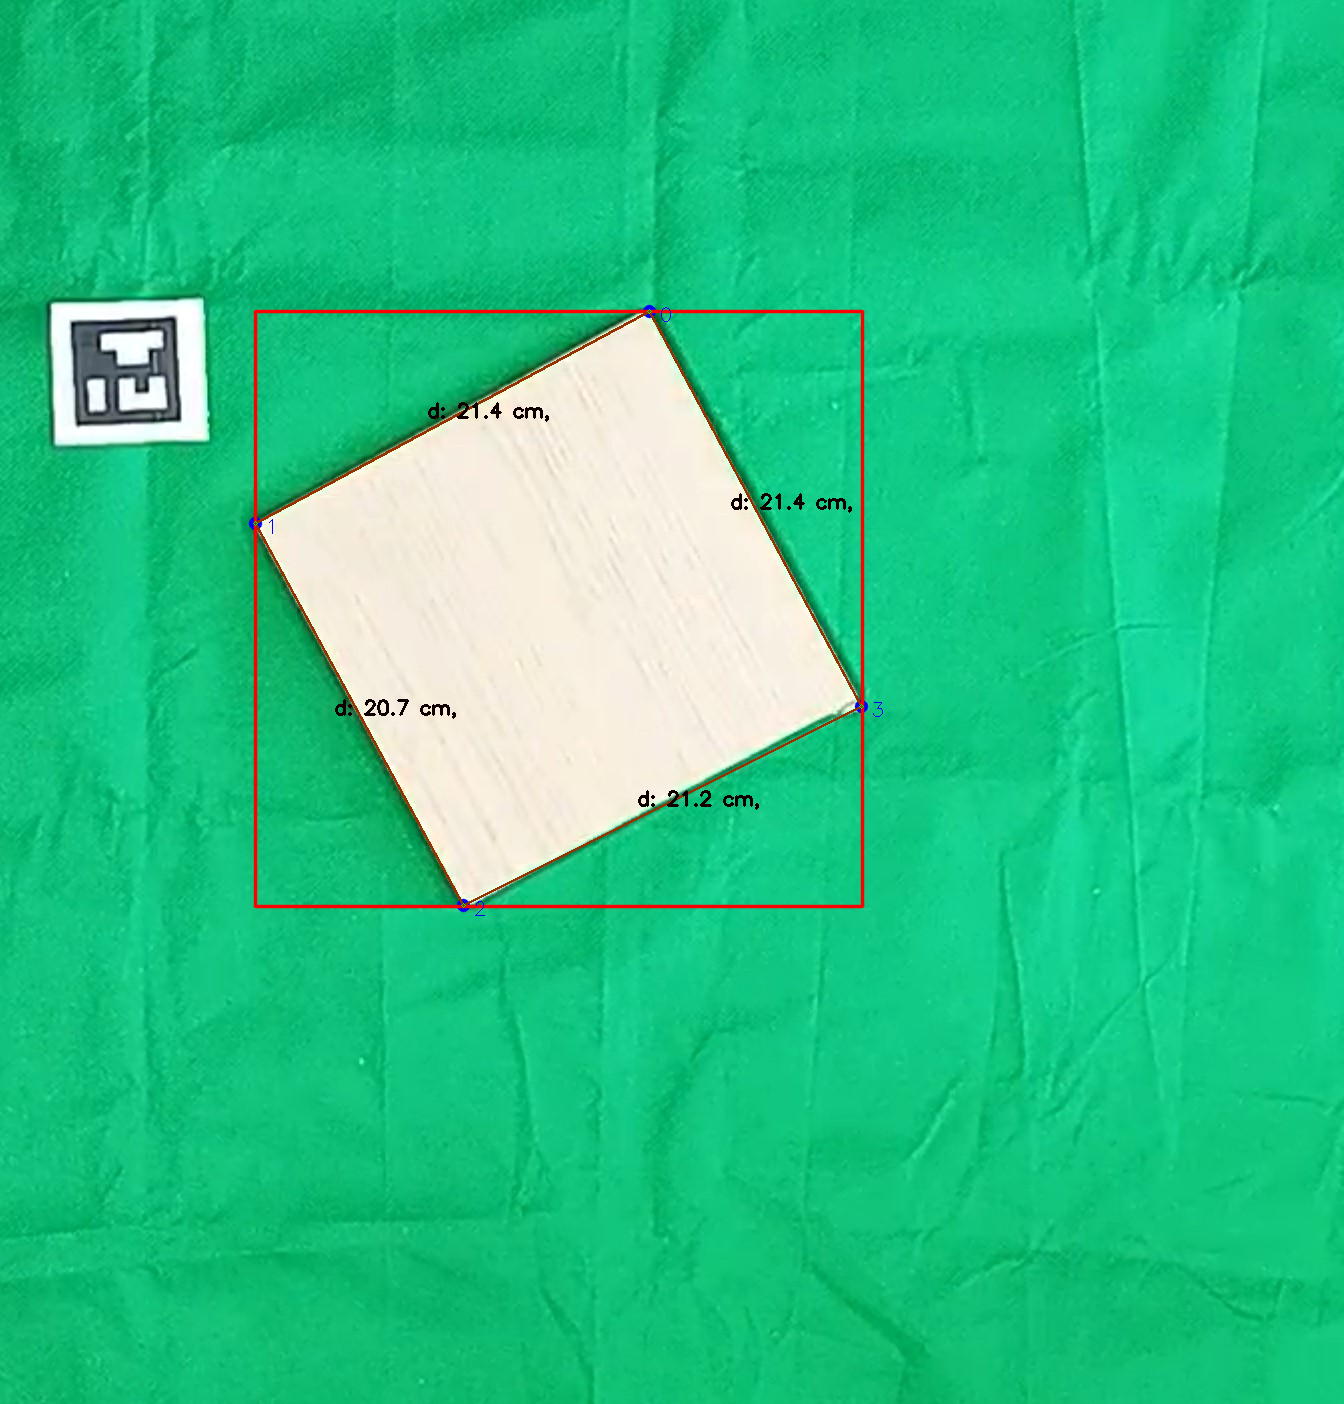
\includegraphics[width=0.35\linewidth]{images/Normal Dist/21.2x21_9.png}
    \caption{Wood Piece with 21.3 x 21.05}
    \label{fig:enter-label}
\end{figure}



\begin{figure}[!h]
    \centering
    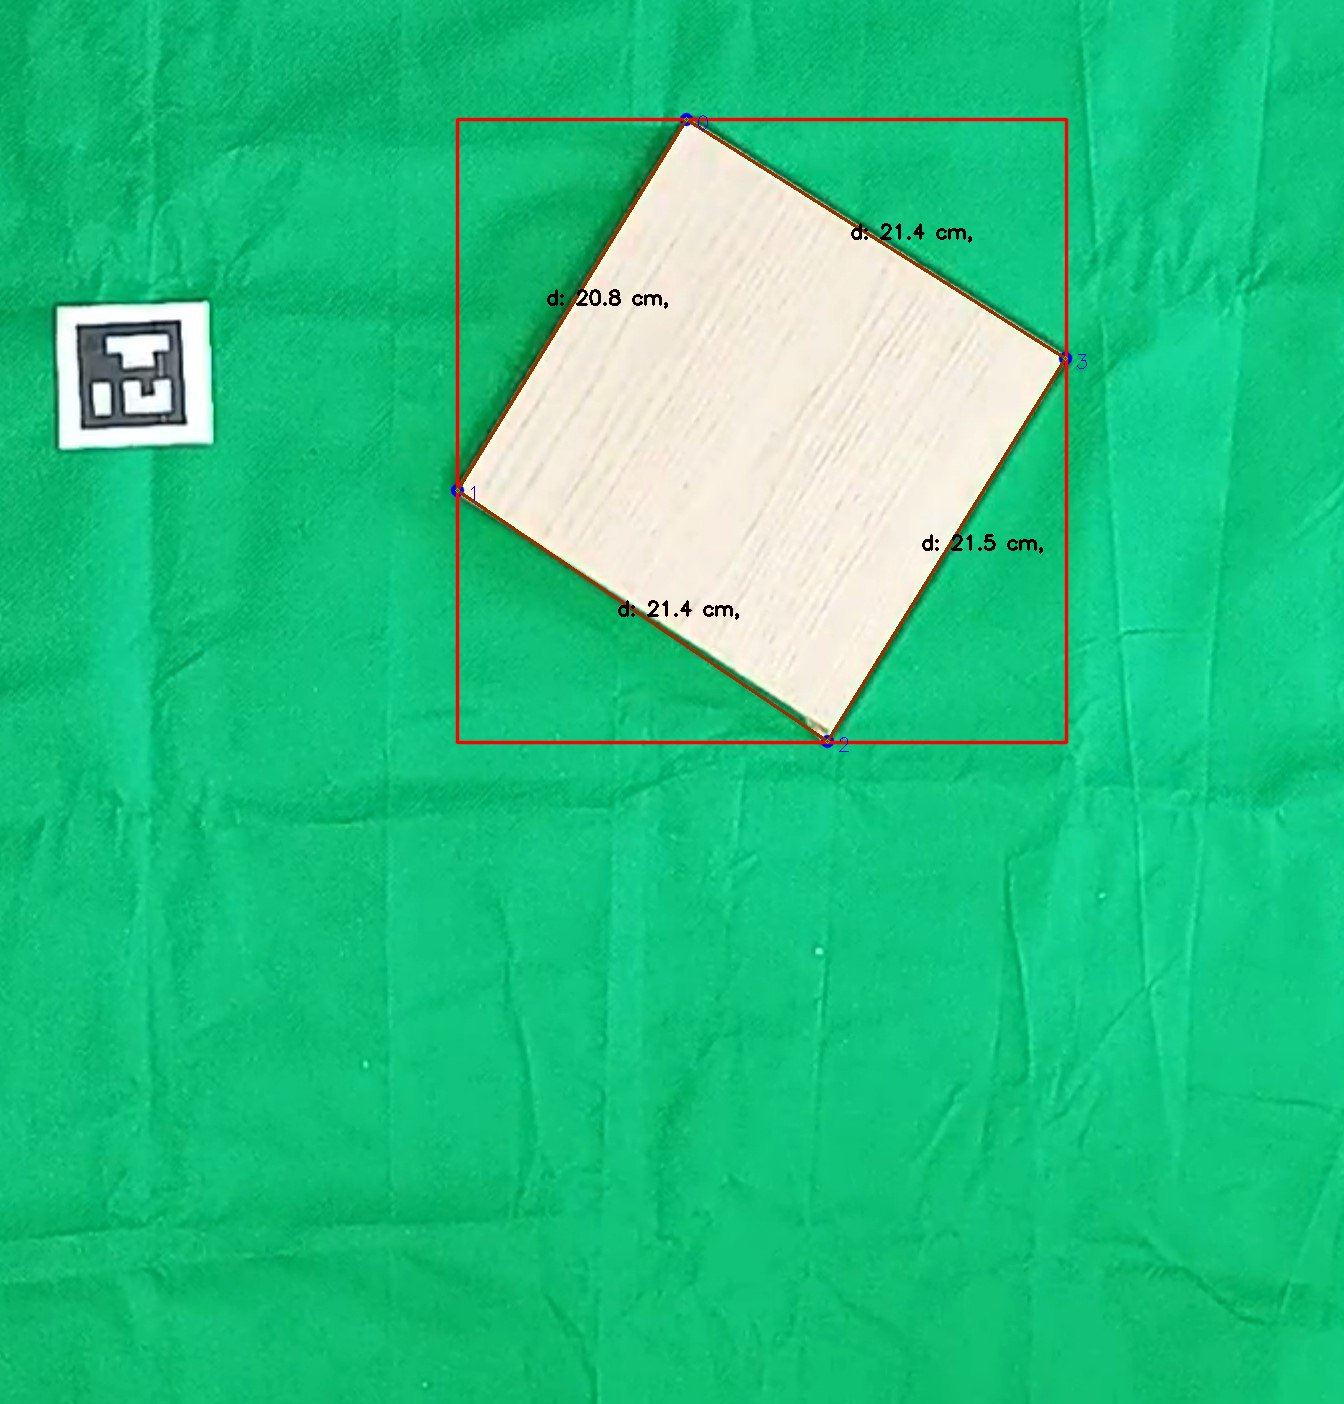
\includegraphics[width=0.35\linewidth]{images/Normal Dist/21.2x21_10.png}
    \caption{Wood Piece with 21.4 x 21.65}
    \label{fig:enter-label}
\end{figure}


\begin{figure}[!h]
    \centering
    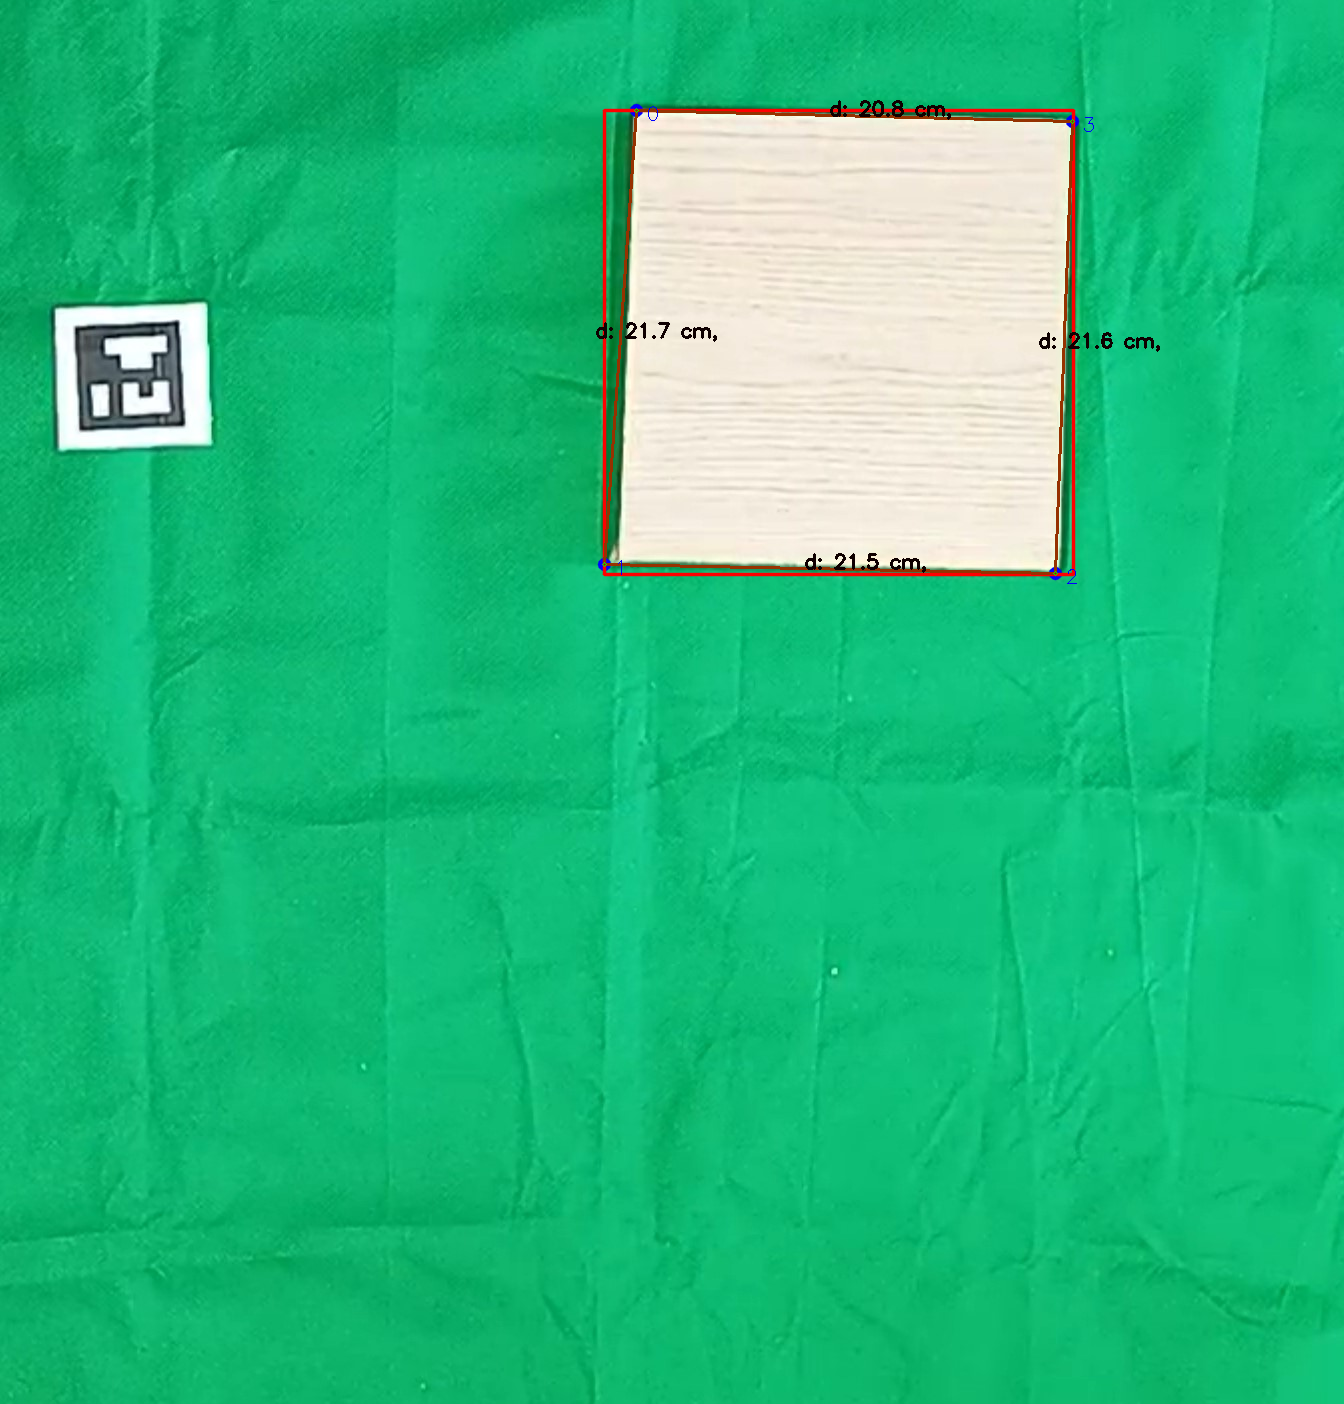
\includegraphics[width=0.35\linewidth]{images/Normal Dist/21.2x21_11.png}
    \caption{Wood Piece with 21.65 x 21.15}
    \label{fig:enter-label}
\end{figure}


\begin{figure}[!h]
    \centering
    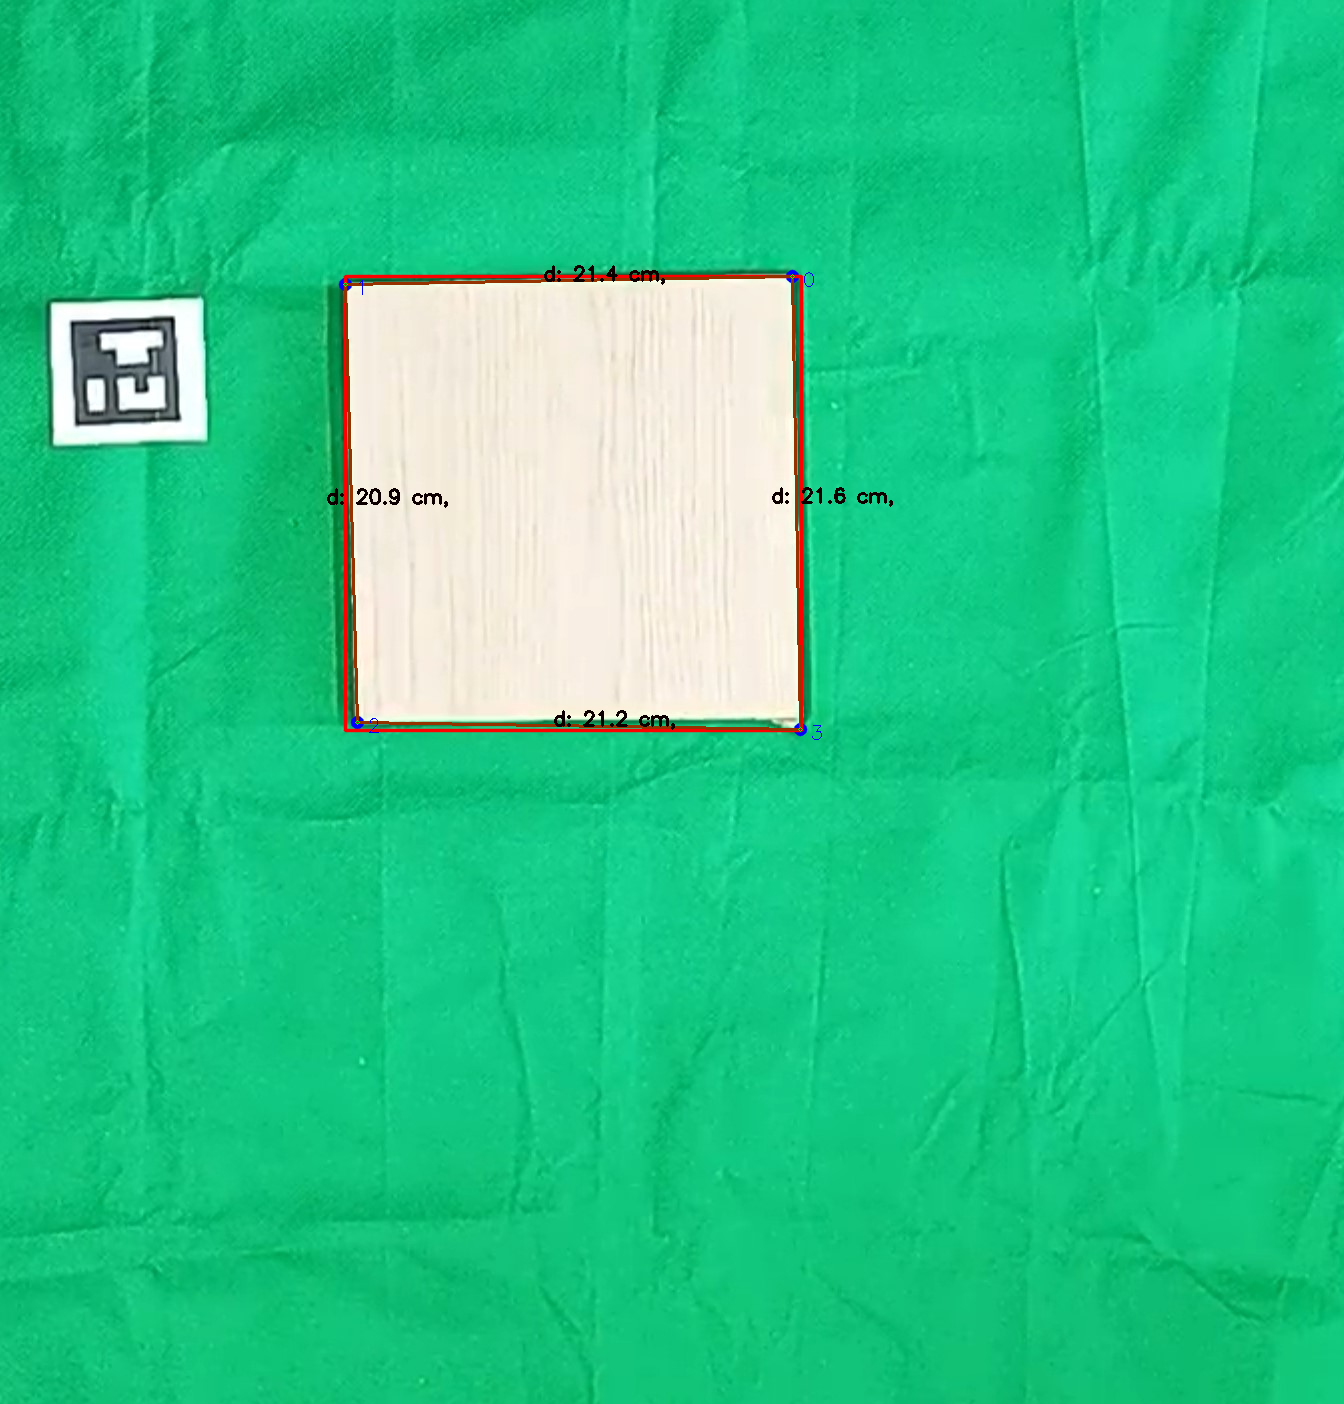
\includegraphics[width=0.35\linewidth]{images/Normal Dist/21.2x21_12.png}
    \caption{Wood Piece with 21.0 x 21.25}
    \label{fig:enter-label}
\end{figure}